\chapter{Training}

%We decided to use the $F_1$ score as metric to evaluate our models.

\section{Network from scratch}

\paragraph{Modus Operandi}
We used the \emph{trial-and-error} approach to create the networks discussed in this chapter, since there are too many hyper-parameters to try.  We started with a small model that did not fit well and then gradually increase
its size until it started to generalize. We also tried to augment the input data by playing with the pictures' contrast in a model but with unimpressive results.

\paragraph{General Architecture}
We opted for a batch size of 32, representing the number of samples considered in each iteration. Following the input layer, we applied normalization using a Rescaling Layer to ensure that each pixel value falls within the $[0,1]$ range. Our choice then led us to employ four convolutional layers, incorporating zero-padding to grant equal significance to every pixel within the image. This approach is valuable because even the border regions hold relevance, despite our efforts to crop the images as extensively as possible. We kept the stride at its default value of 1 to avoid any adverse impact on accuracy. Our activation functions of choice were ReLU, defined as $f(x) = \max\{0, x\}$. For the size of the local receptive fields, we stuck with the default 3x3 dimensions.

In the initial convolutional layer, we utilized 32 filters, with a doubling of filter count for each subsequent convolutional layer. To enhance feature extraction, we applied max-pooling after each convolutional layer, thereby consolidating small regions into a single value.

\subsection{One dense layers}
\label{scratch.1dense}

\paragraph{Architecture}
We used one dense layer with 64 neurons. To fight  overfit we used dropout

\lstinputlisting[language=Python,linerange={31-44}]{../train_scratch.py}

\paragraph{Results}
On the validation dataset, we obtained an accuracy $A_\text{val} = 0.91$ and the following $F_1$ scores:

\vspace{5mm}
\begin{tabular}{l|r}%
	\bfseries Class & \bfseries $F_1$% specify table head
	\csvreader[head to column names]{assets/results/preMELD.scratch/model.1dense/f1.csv}{}% use head of csv as column names
	{\\\hline \class & \csvcolii}% specify your coloumns here
\end{tabular}
\vspace{5mm}

\begin{figure}[H]
	\centering
	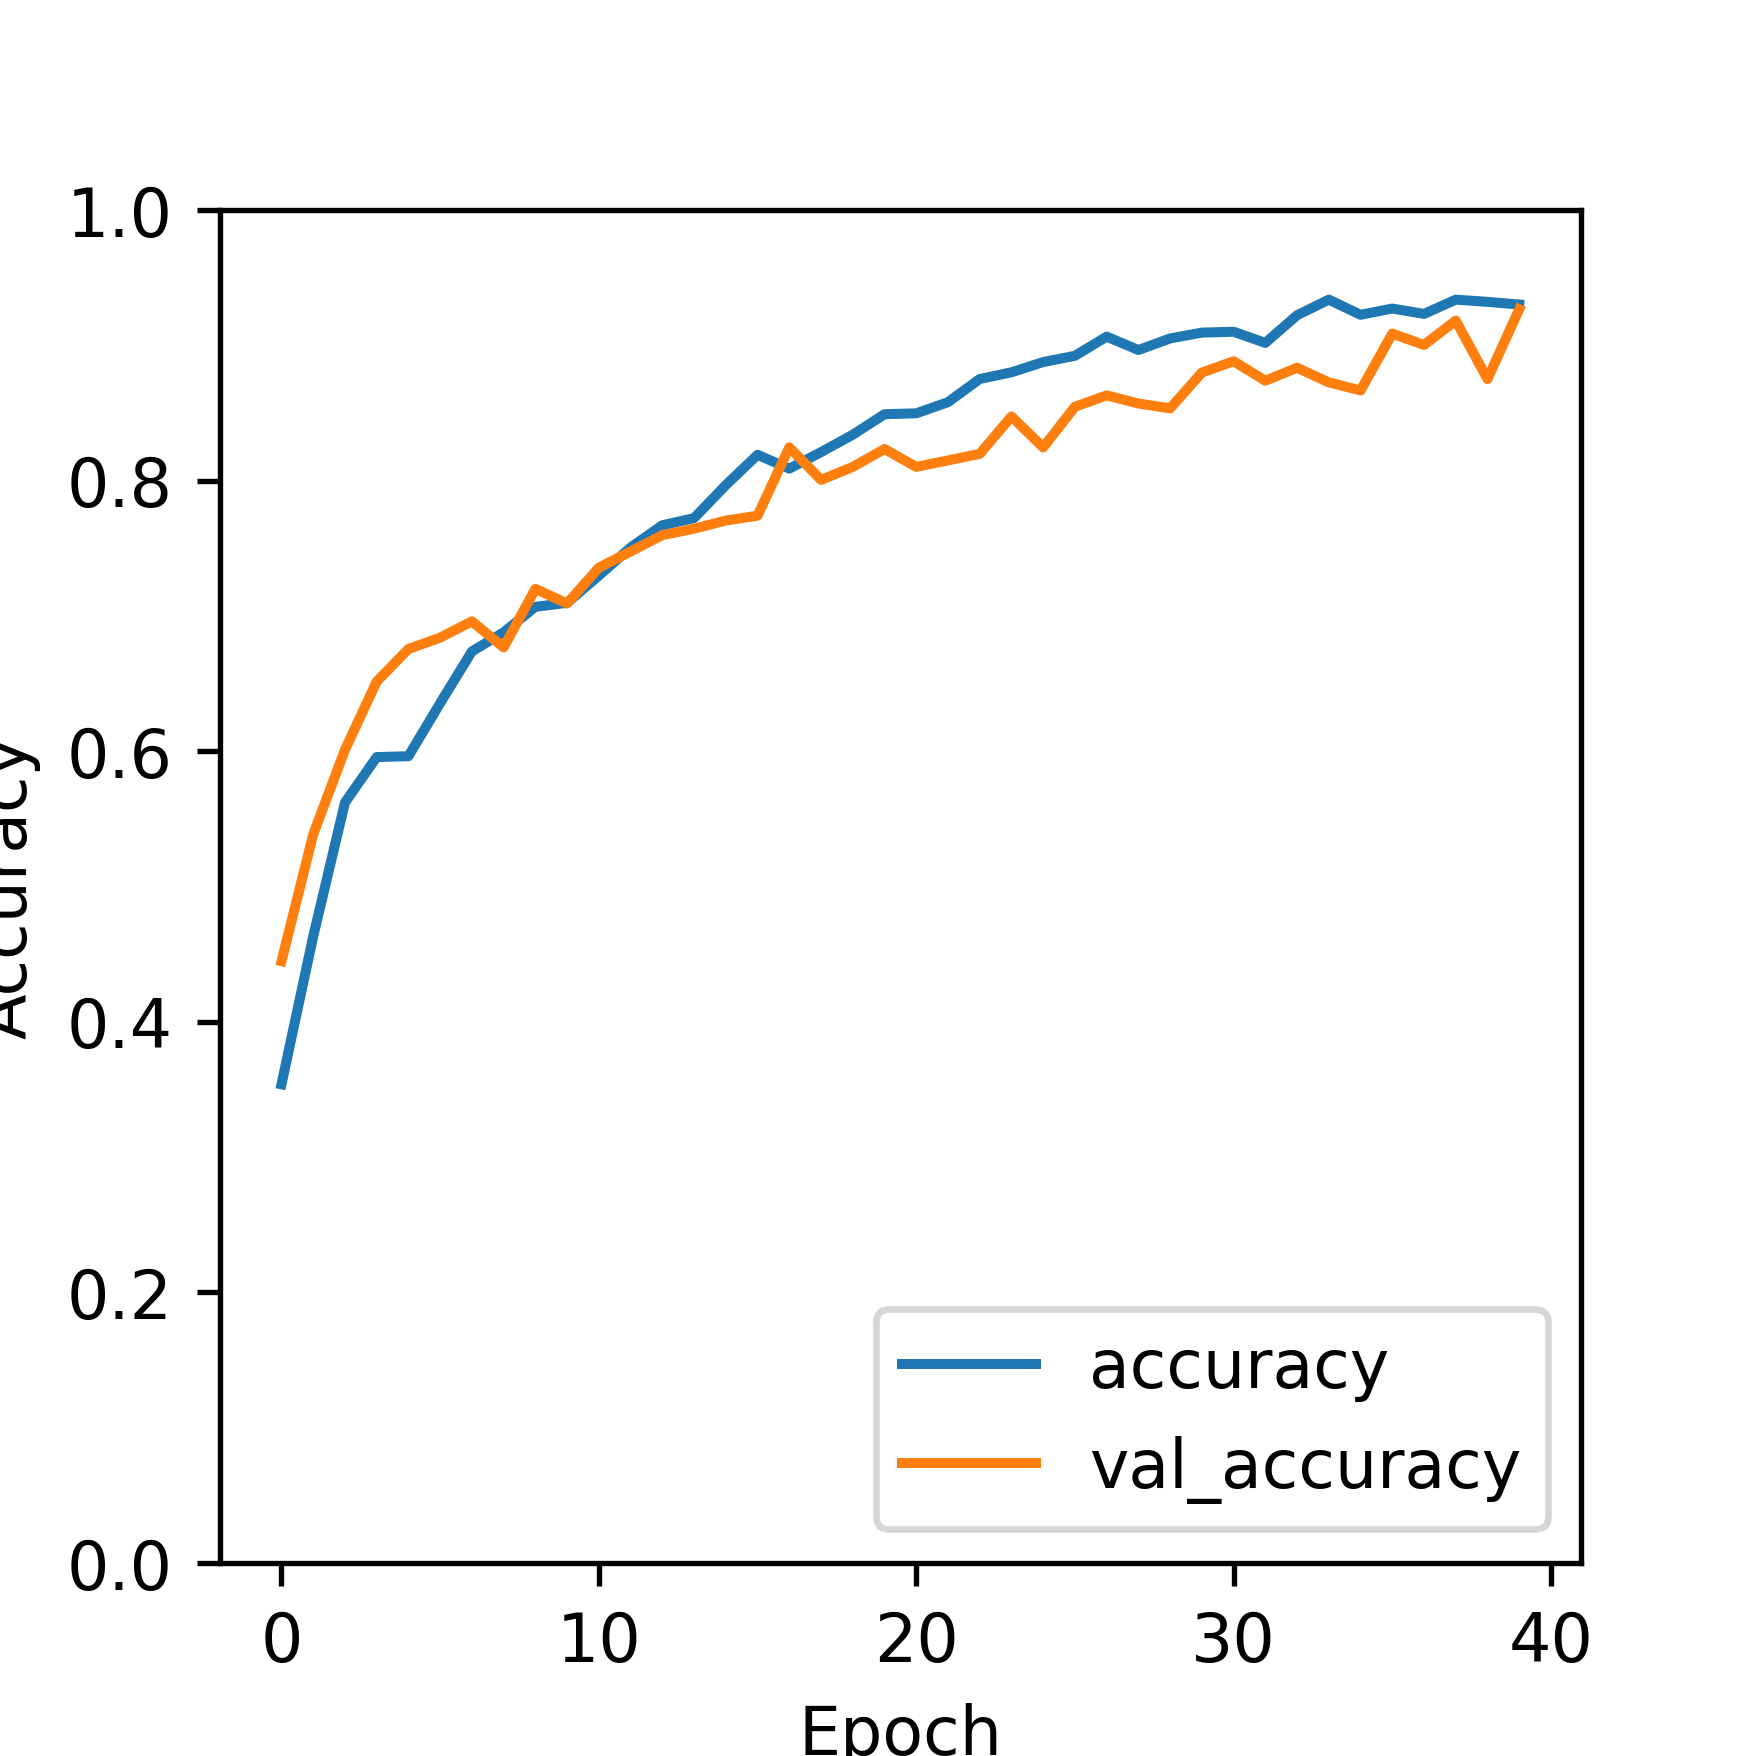
\includegraphics[width=.5\textwidth]{assets/results/preMELD.scratch/model.1dense/learning_history-acc.png}\hfill
	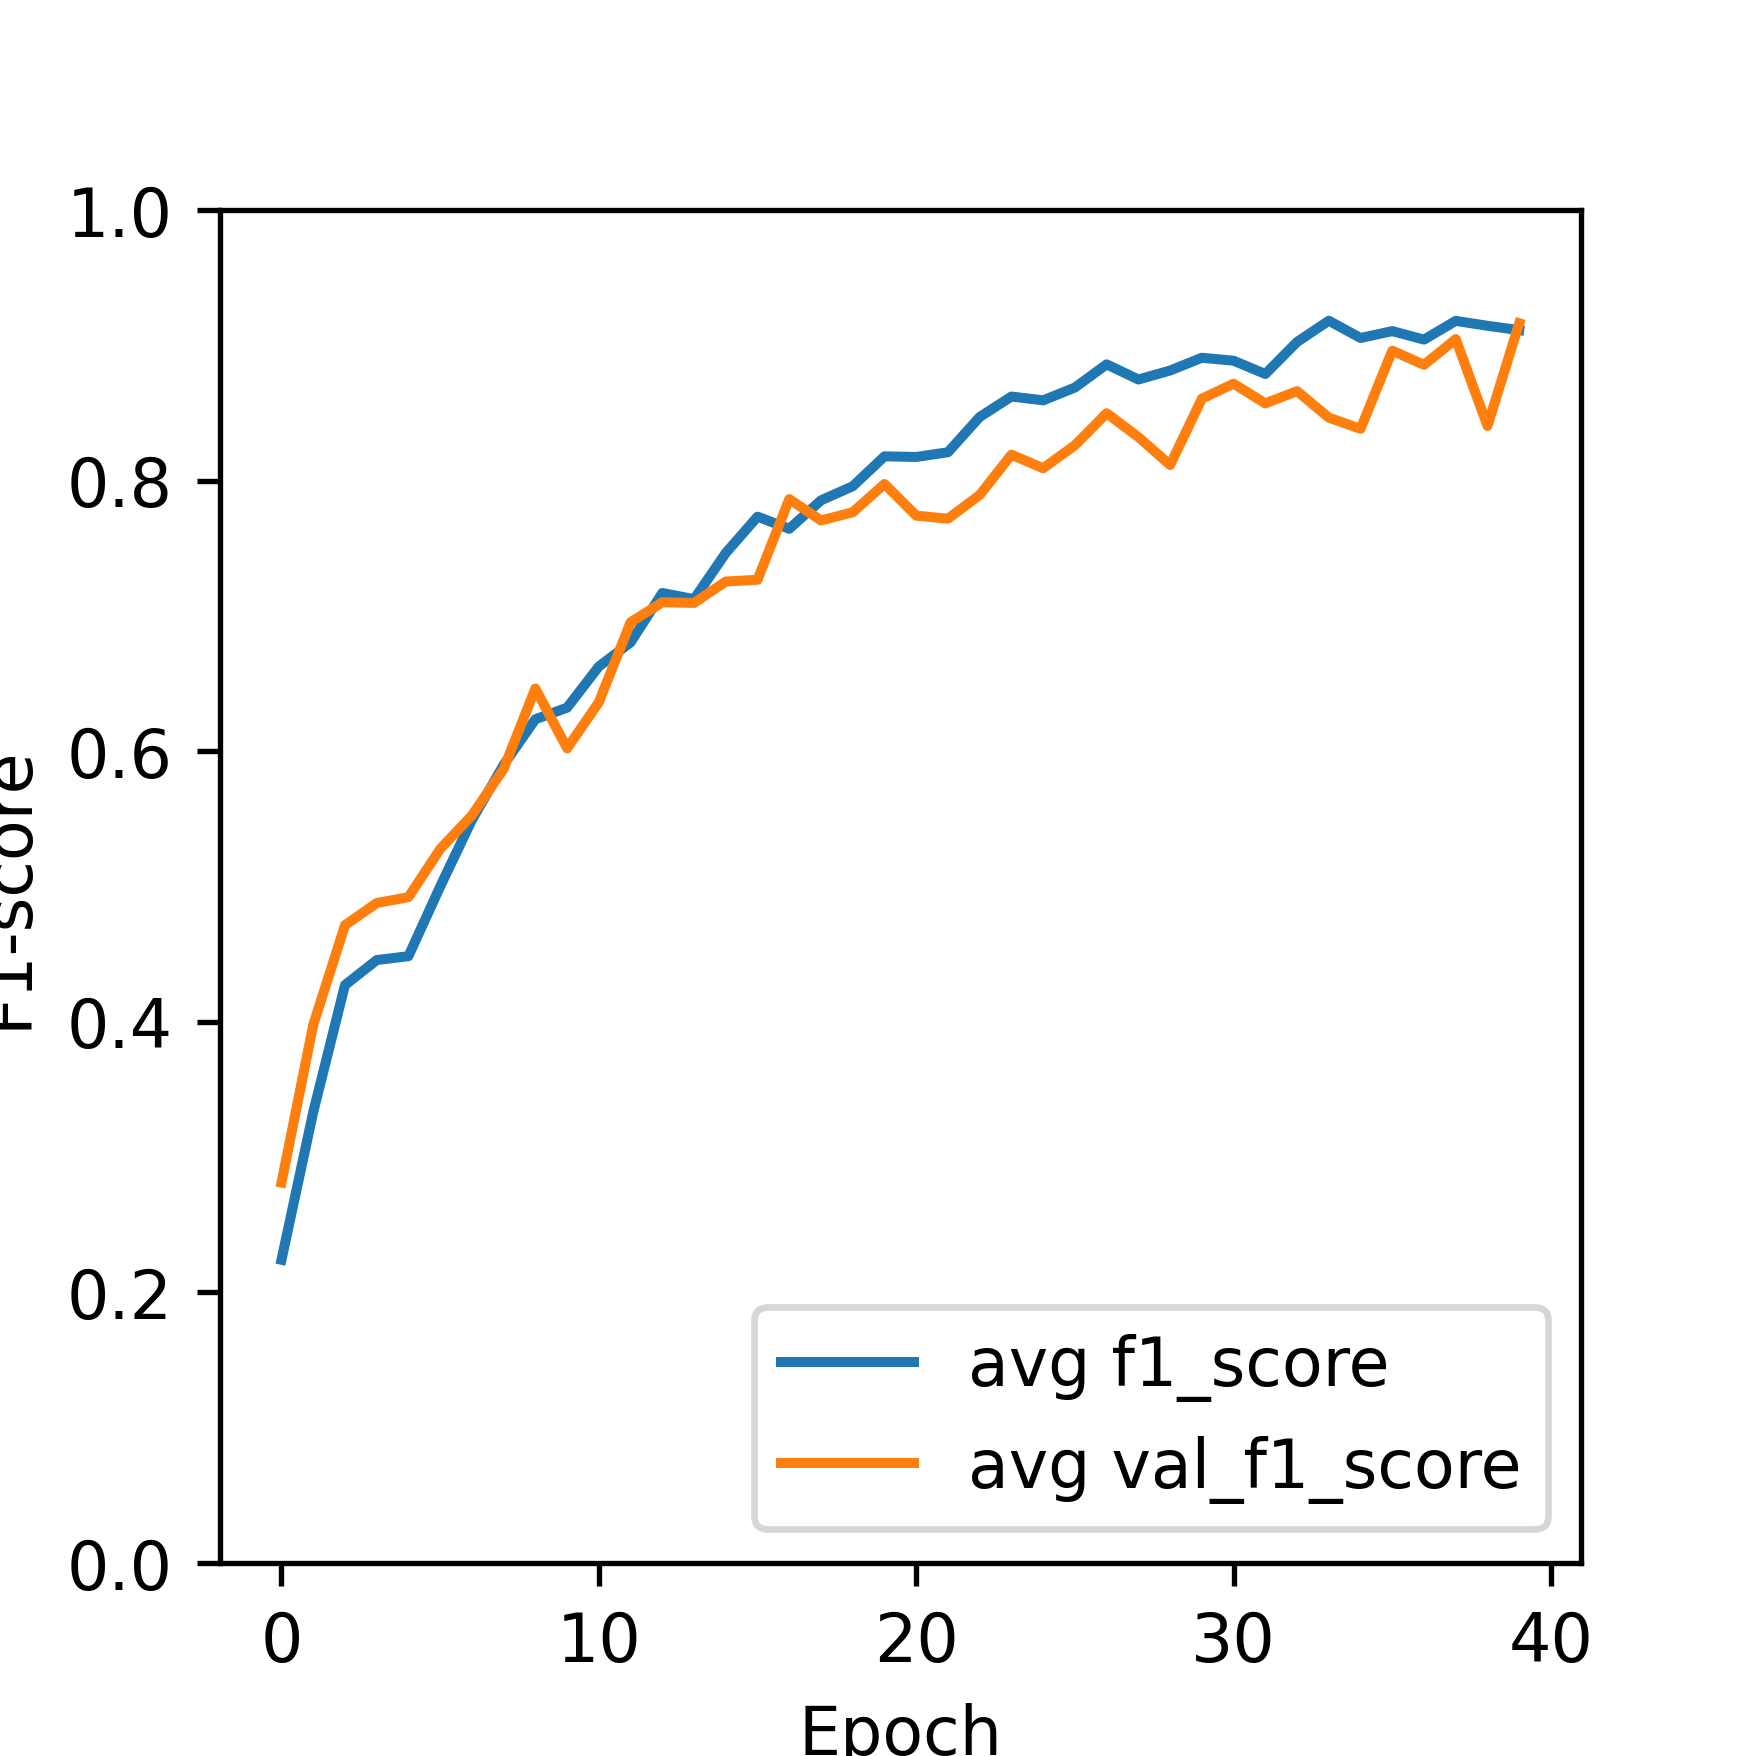
\includegraphics[width=.5\textwidth]{assets/results/preMELD.scratch/model.1dense/learning_history-f1_score.png}\hfill
	\caption{$F_1$ figures are from average from all $F_1^c$}
	\label{fig:figure2}
\end{figure}

\begin{figure}[H]
	\centering
	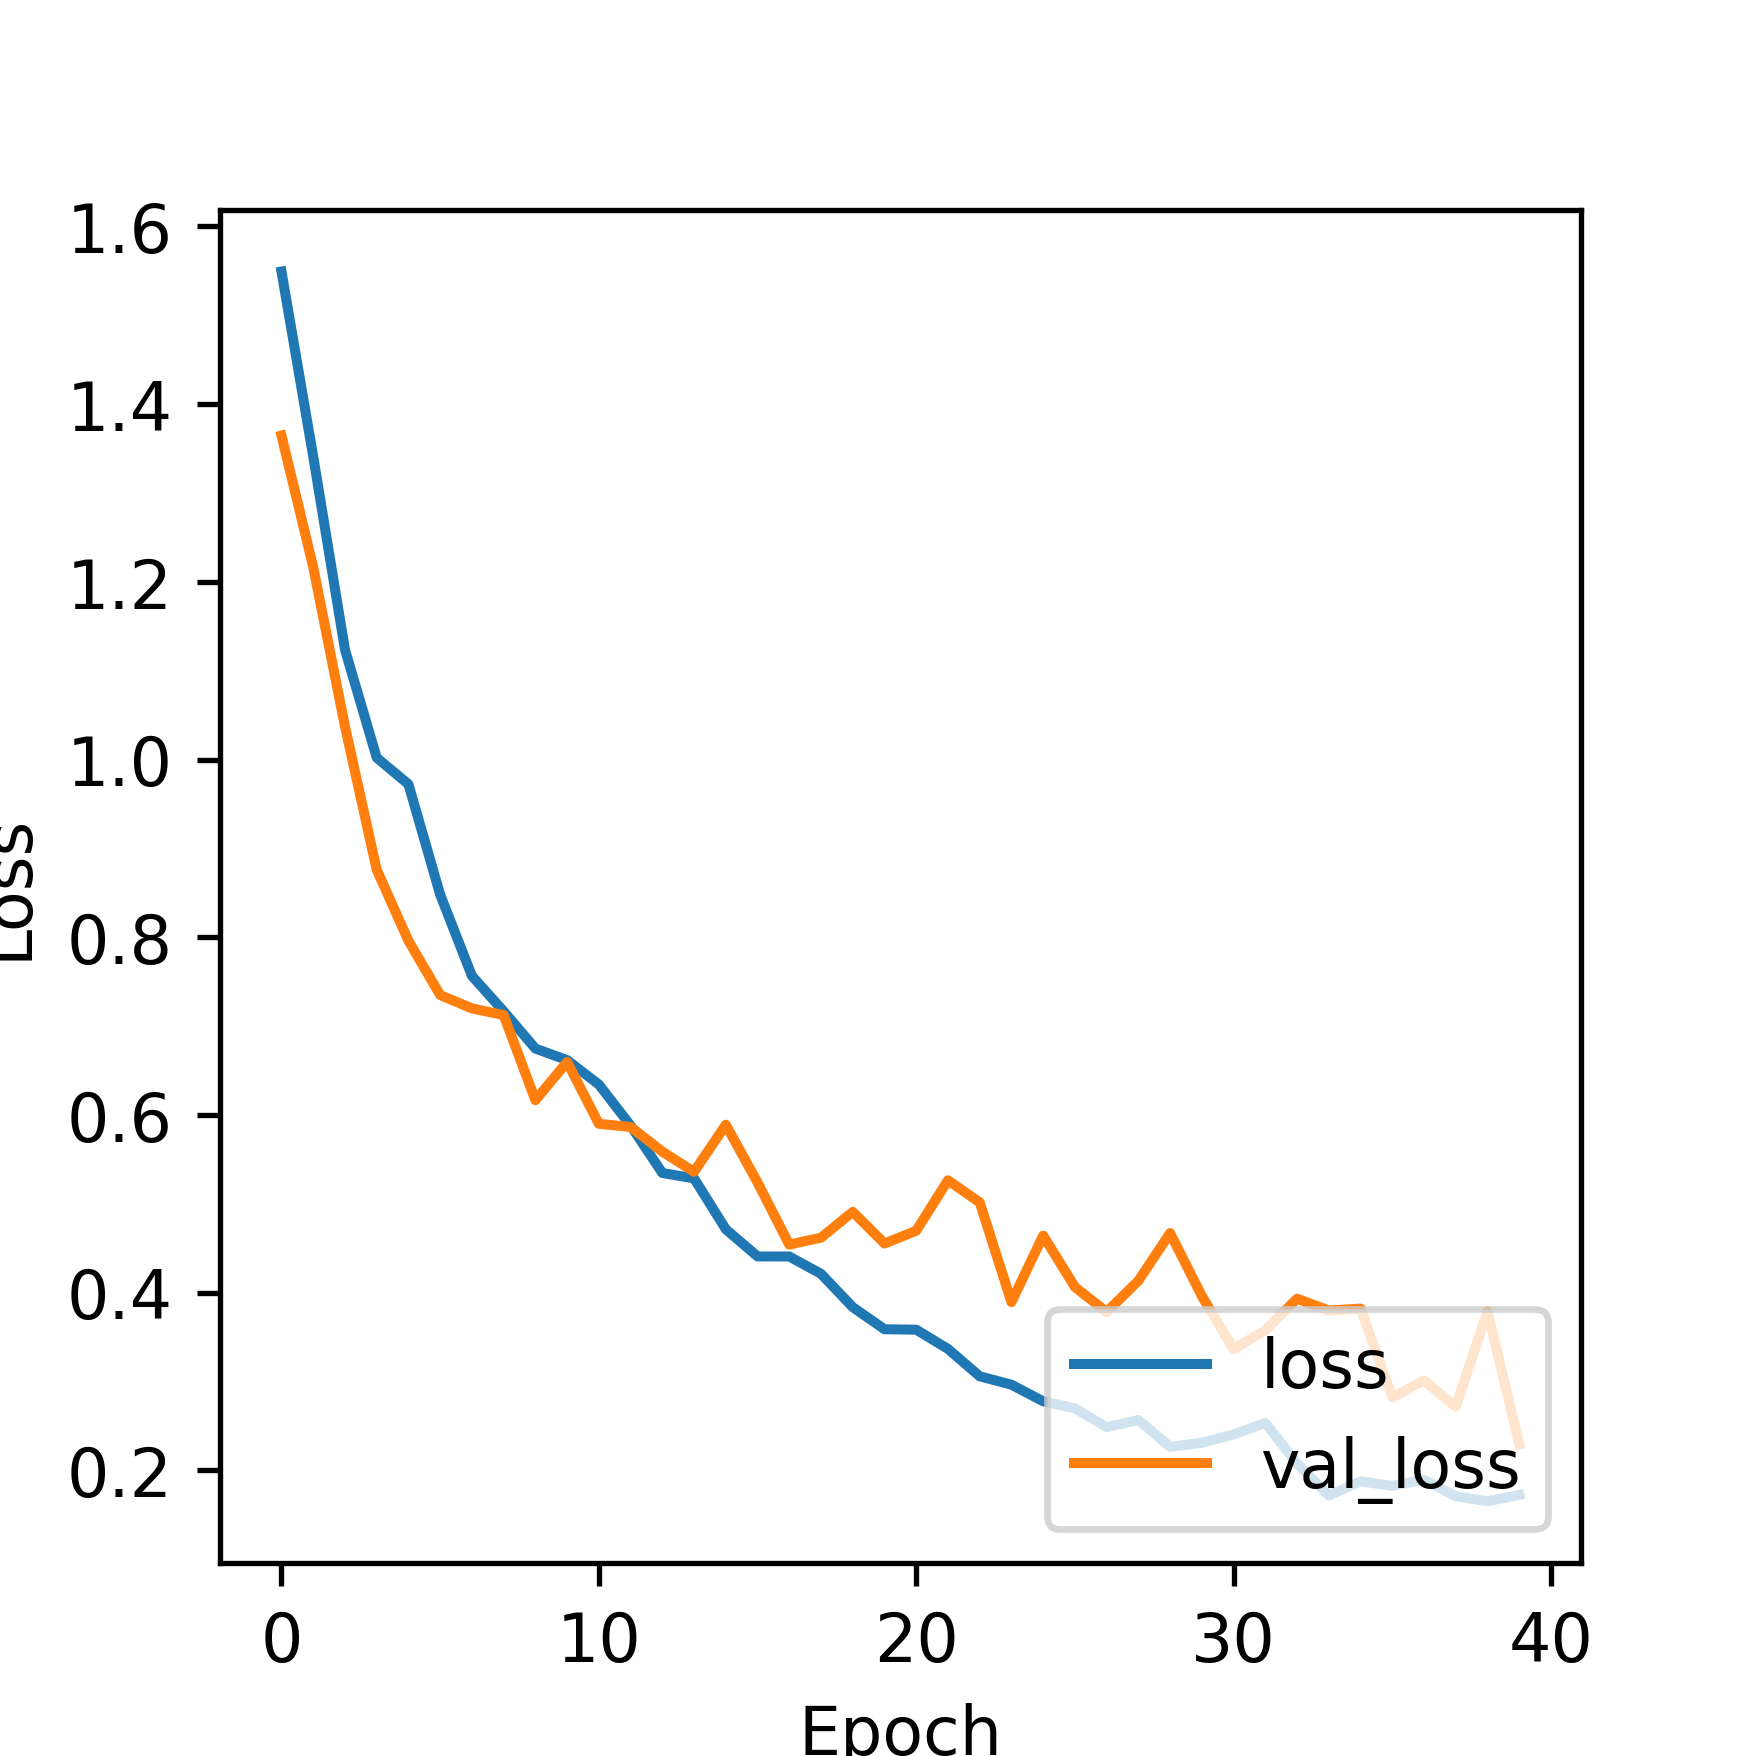
\includegraphics[width=.5\textwidth]{assets/results/preMELD.scratch/model.1dense/learning_history-loss.png}
	
	\label{fig:figure3}
\end{figure}

\begin{figure}[H]
	\centering
	\includegraphics[width=.95\textwidth]{assets/results/preMELD.scratch/model.1dense/confusion_matrix.png}
	
	\label{fig:cm1}
\end{figure}




\subsection{Two dense layers}
\label{scratch.2dense}

\paragraph{Architecture}
We used two dense layers with 128 and 256 neurons. To fight overfit used dropout as well as \emph{L1L2} regularization.

\lstinputlisting[language=Python,linerange={51-73}]{../train_scratch.py}

\paragraph{Results}
On the validation dataset, we obtained an accuracy $A_\text{val} = 0.91$ and the following $F_1$ scores:

\vspace{5mm}
\begin{tabular}{l|r}%
	\bfseries Class & \bfseries $F_1$% specify table head
	\csvreader[head to column names]{assets/results/preMELD.scratch/model.2dense/f1.csv}{}% use head of csv as column names
	{\\\hline \class & \csvcolii}% specify your coloumns here
\end{tabular}
\vspace{5mm}

\begin{figure}[H]
	\centering
	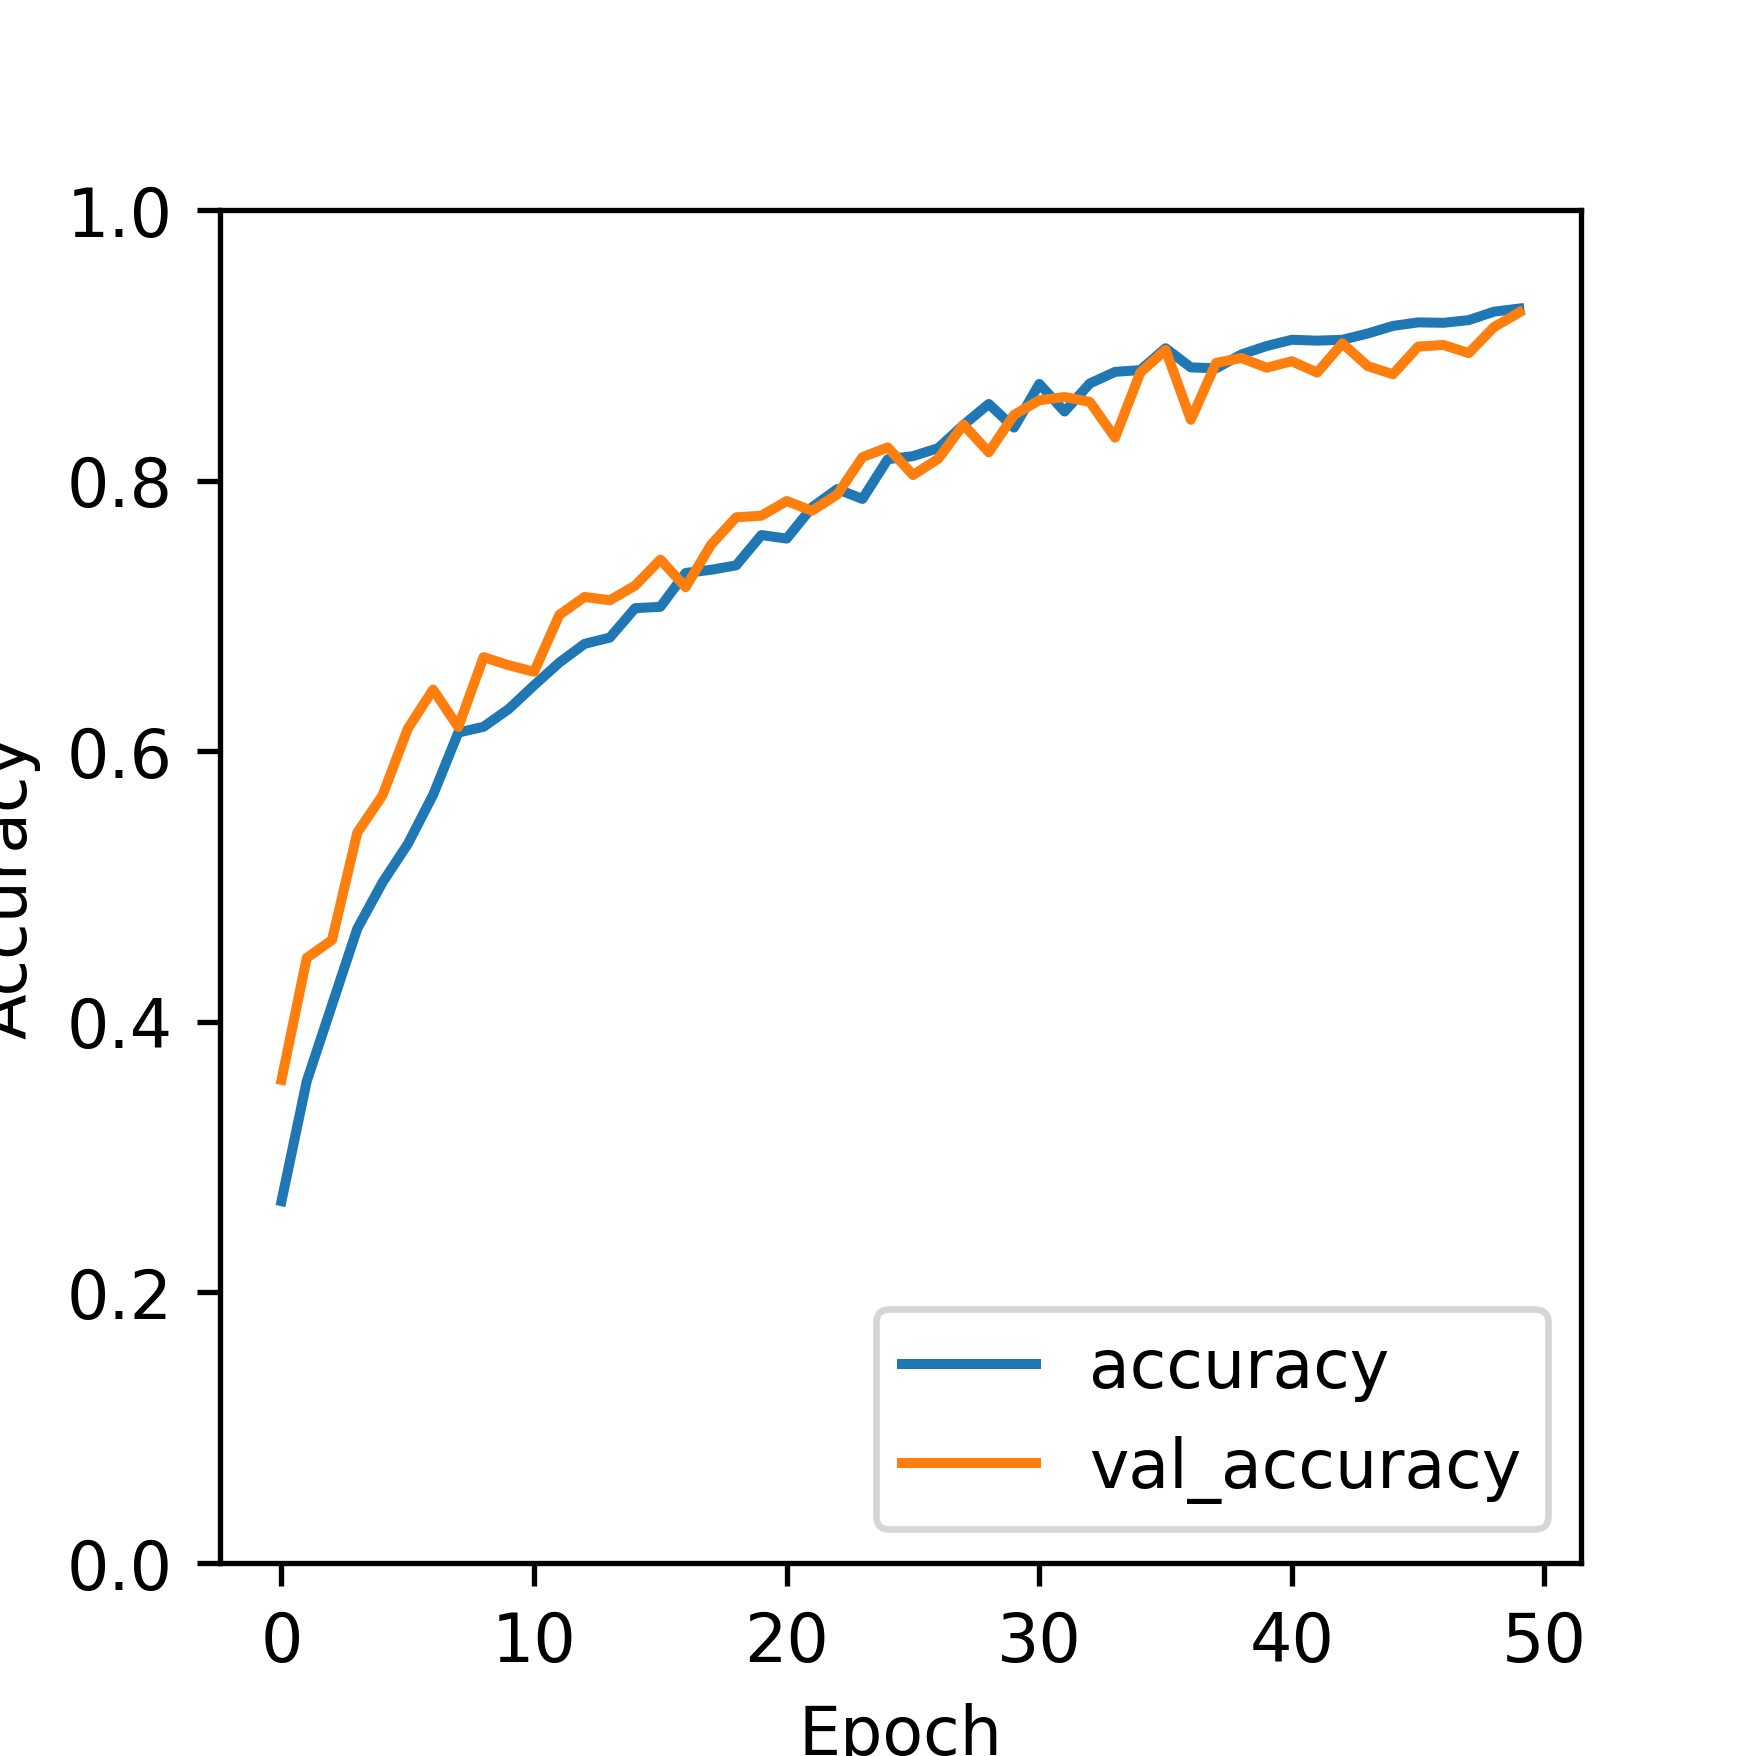
\includegraphics[width=.5\textwidth]{assets/results/preMELD.scratch/model.2dense/learning_history-acc.png}\hfill
	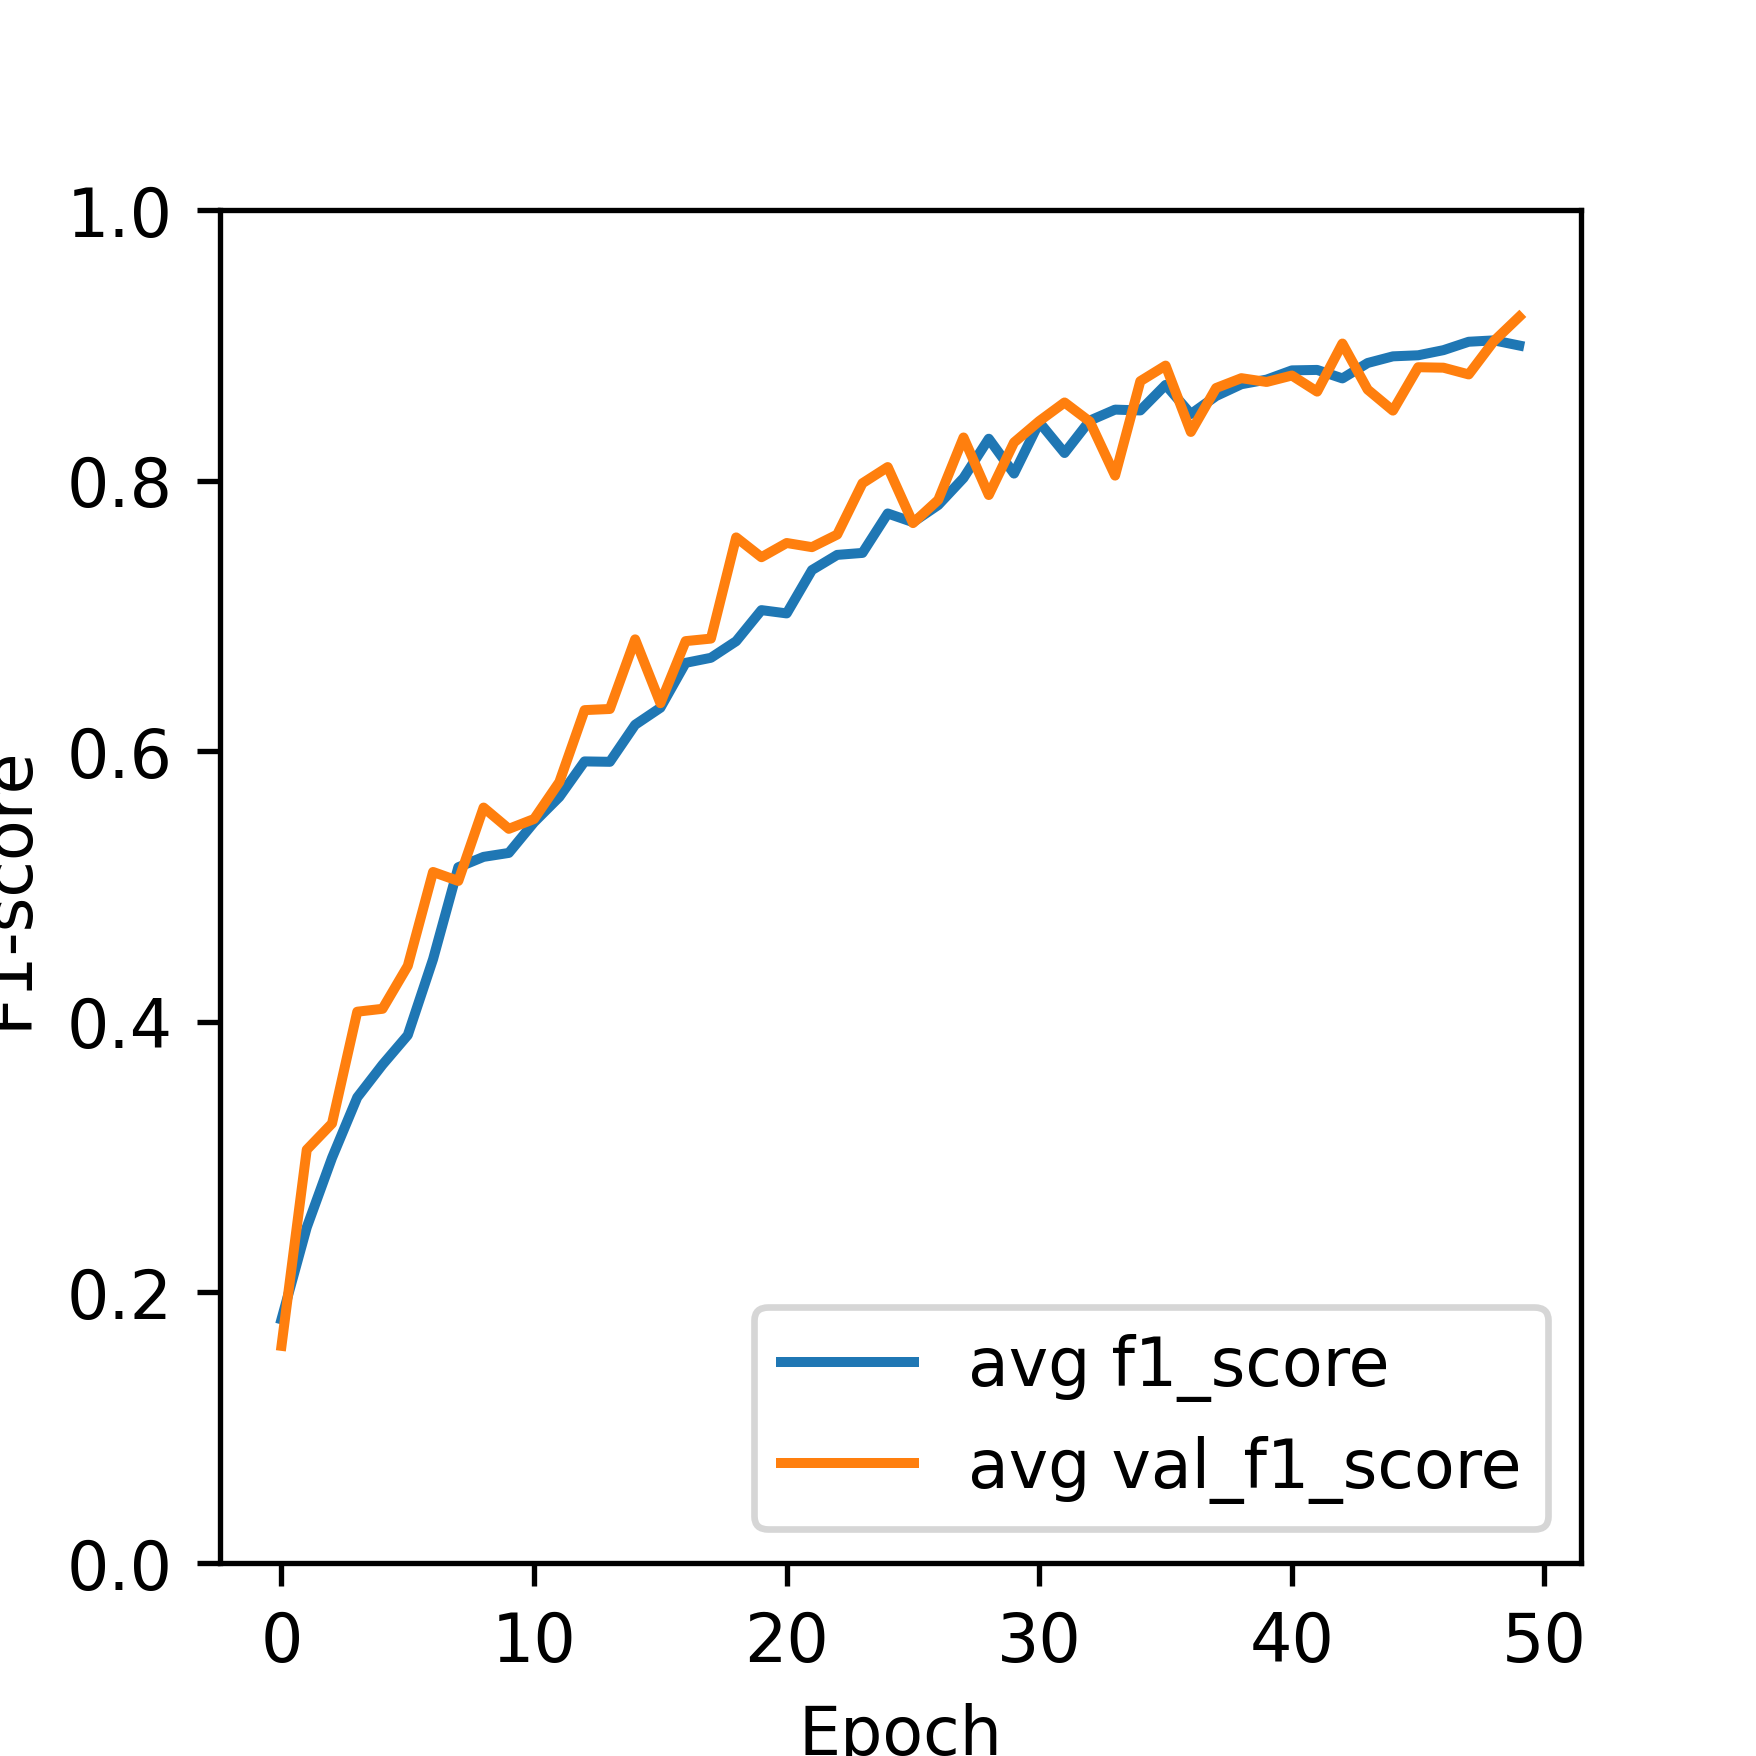
\includegraphics[width=.5\textwidth]{assets/results/preMELD.scratch/model.2dense/learning_history-f1_score.png}\hfill
	\caption{$F_1$ figures are from average from all $F_1^c$}
	\label{fig:figure4}
\end{figure}

\begin{figure}[H]
	\centering
	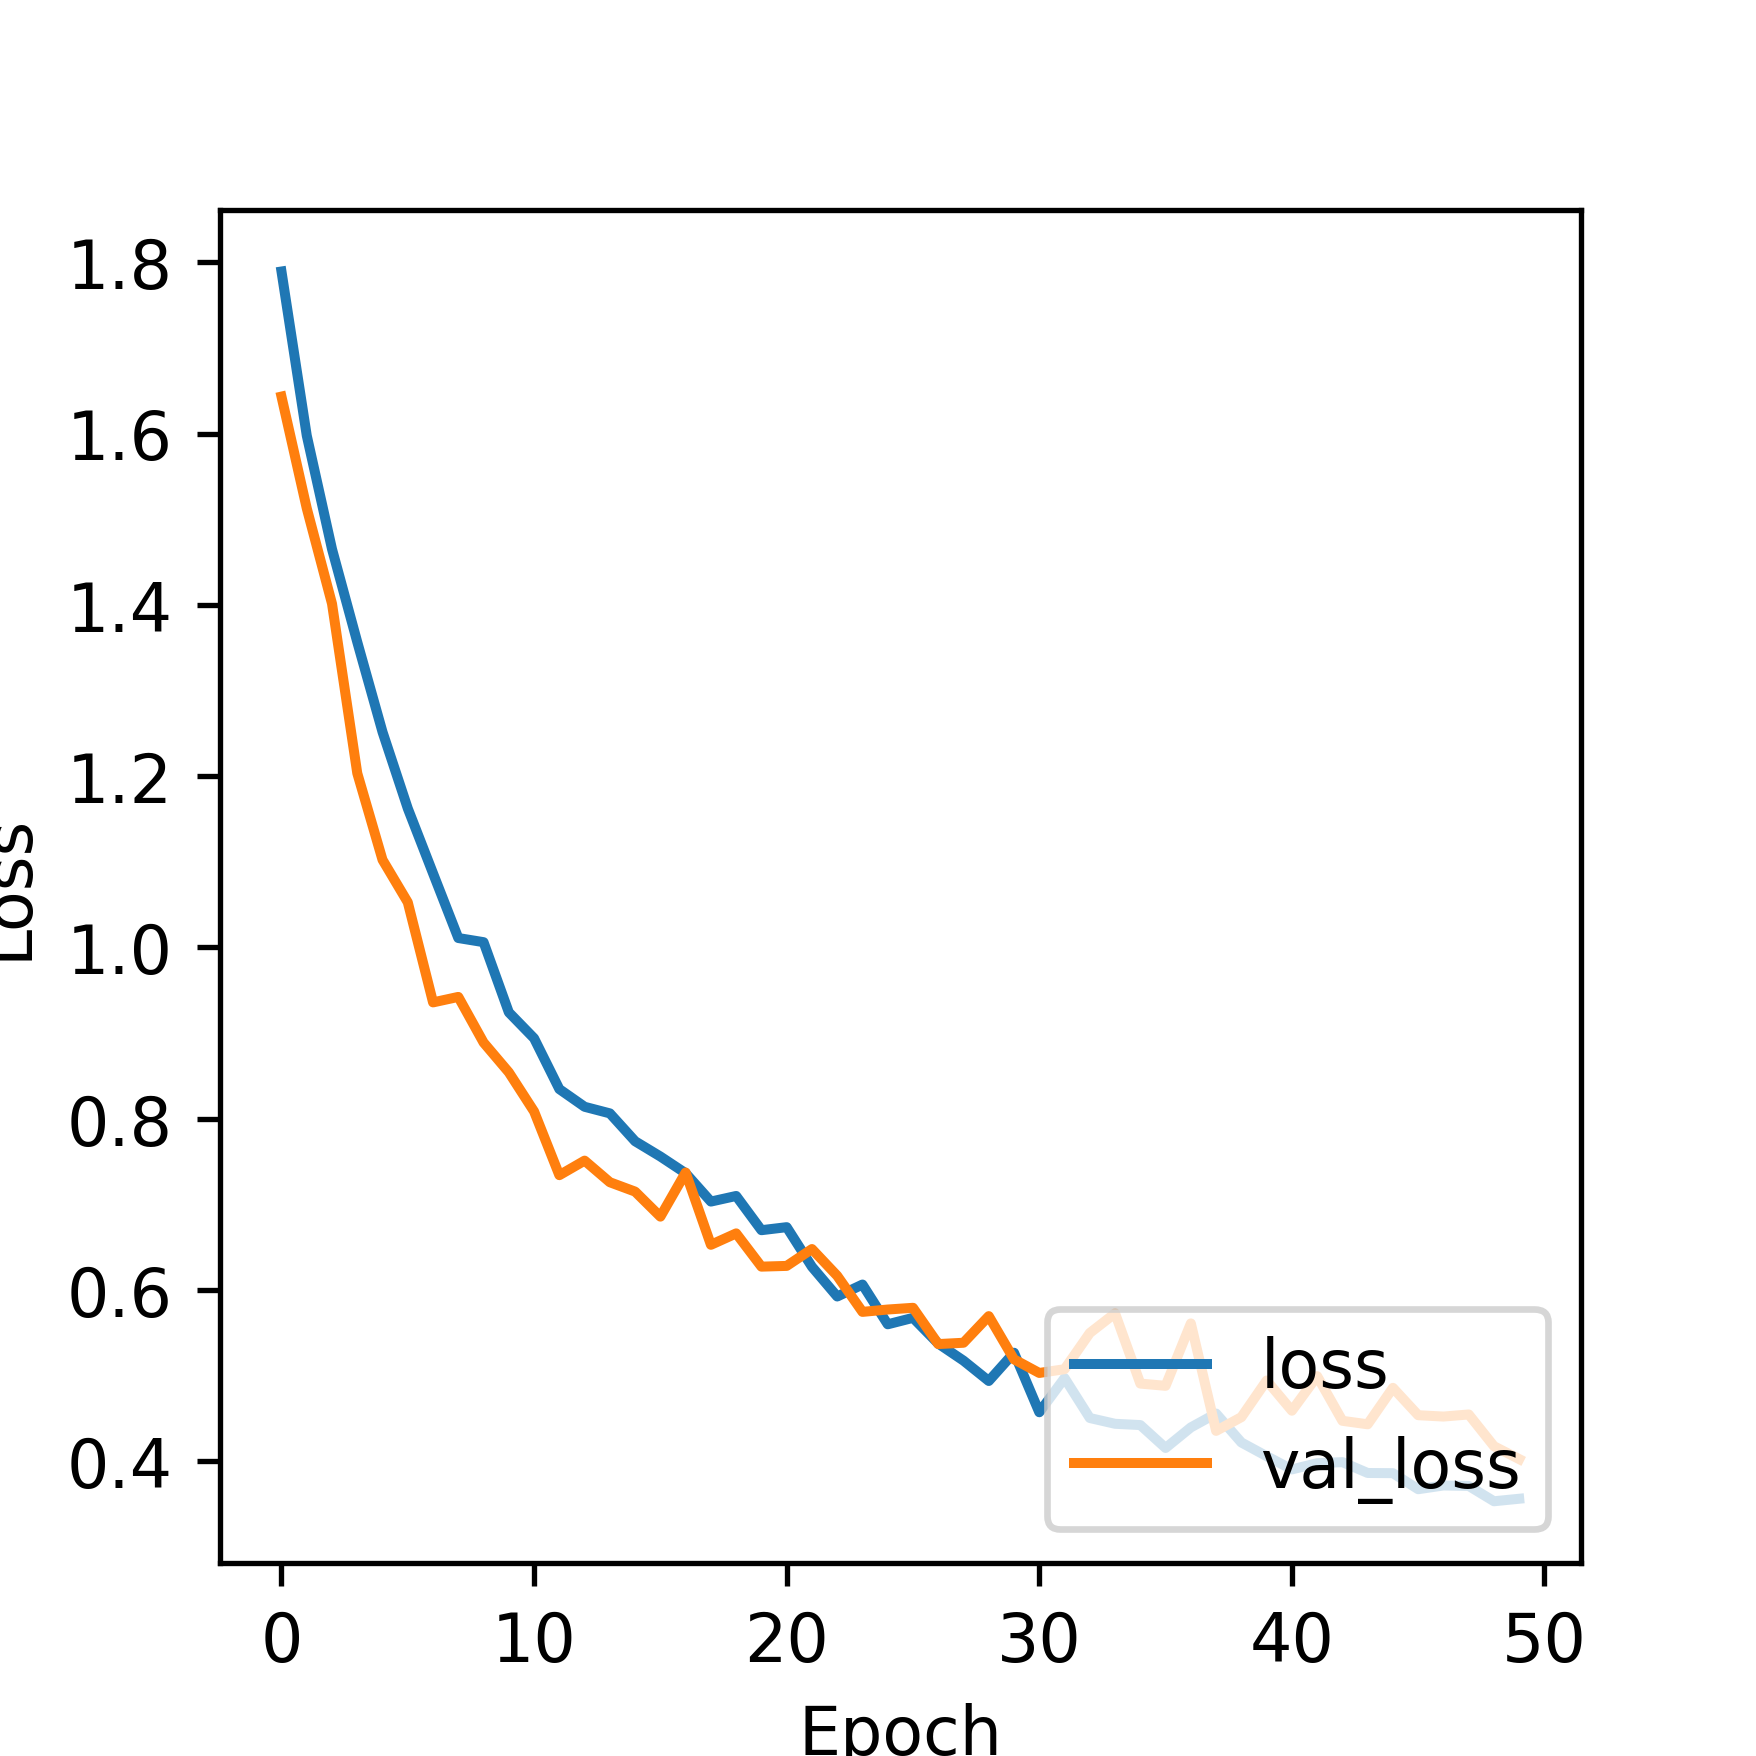
\includegraphics[width=.5\textwidth]{assets/results/preMELD.scratch/model.2dense/learning_history-loss.png}
	
	\label{fig:figure5}
\end{figure}

\begin{figure}[H]
	\centering
	\includegraphics[width=.95\textwidth]{assets/results/preMELD.scratch/model.2dense/confusion_matrix.png}
	
	\label{fig:cm2}
\end{figure}





\subsection{Three dense layers}

\paragraph{Architecture}
We used three dense layers with 2048, 1024 and 512 neurons. Given the high number of weight we used higher dropouts and \emph{L1L2} regularization.

\lstinputlisting[language=Python,linerange={121-142}]{../train_scratch.py}

\paragraph{Results}
On the validation dataset, we obtained an accuracy $A_\text{val} = 0.83$ and the following $F_1$ scores:

\vspace{5mm}
\begin{tabular}{l|r}%
	\bfseries Class & \bfseries $F_1$% specify table head
	\csvreader[head to column names]{assets/results/preMELD.scratch/model.3dense/f1.csv}{}% use head of csv as column names
	{\\\hline \class & \csvcolii}% specify your coloumns here
\end{tabular}
\vspace{5mm}

\begin{figure}[H]
	\centering
	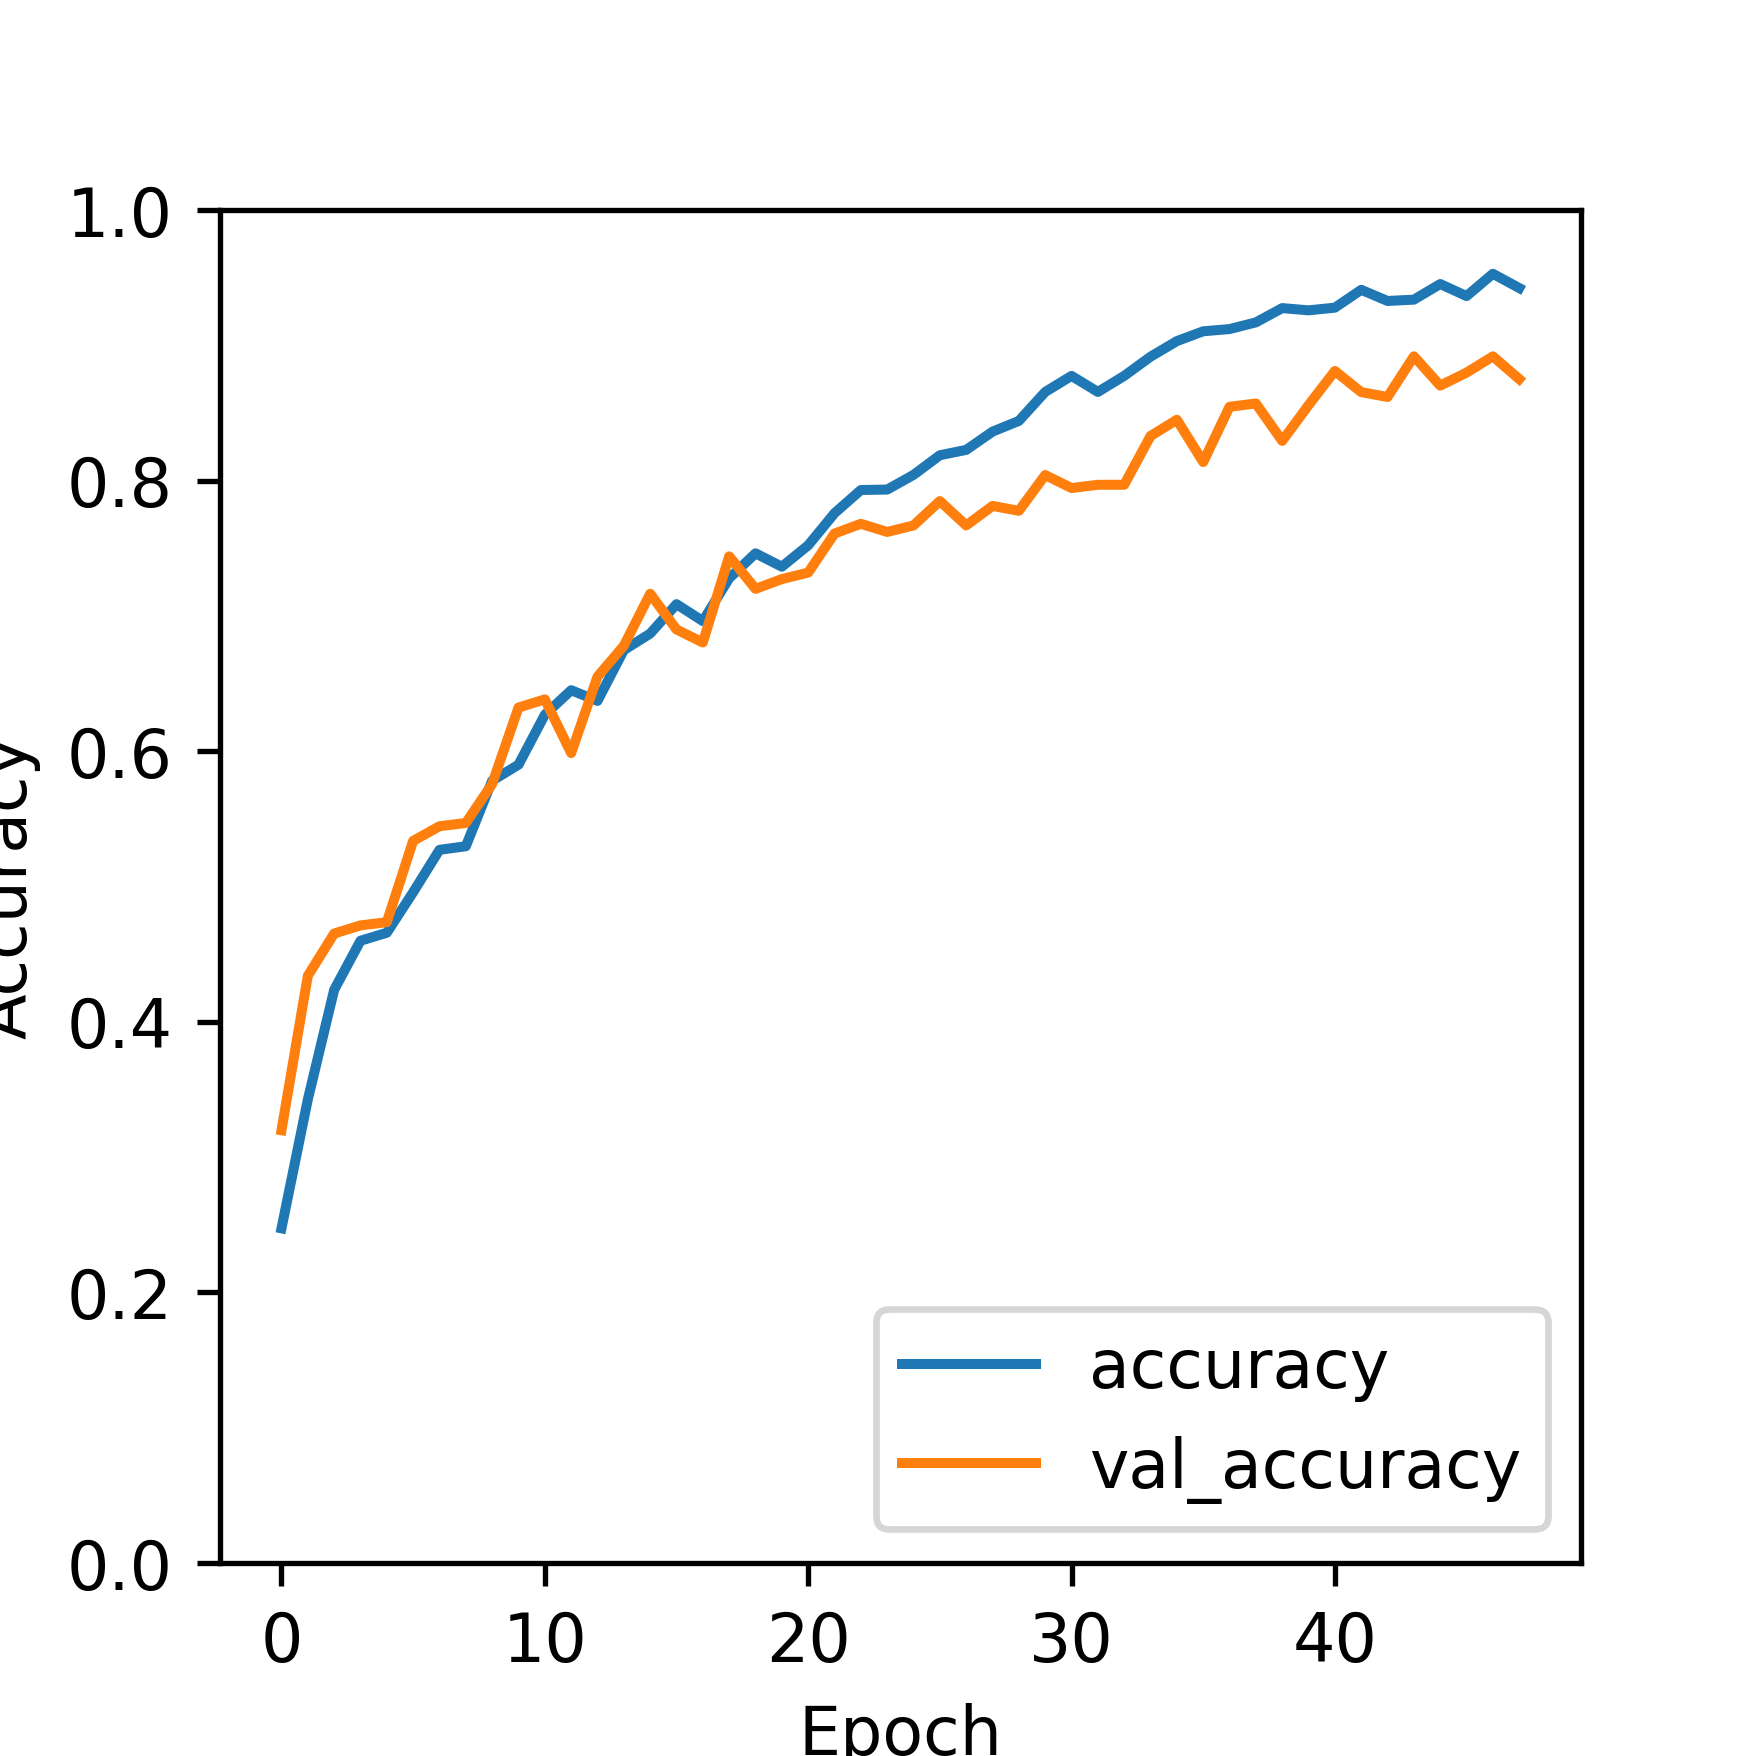
\includegraphics[width=.5\textwidth]{assets/results/preMELD.scratch/model.3dense/learning_history-acc.png}\hfill
	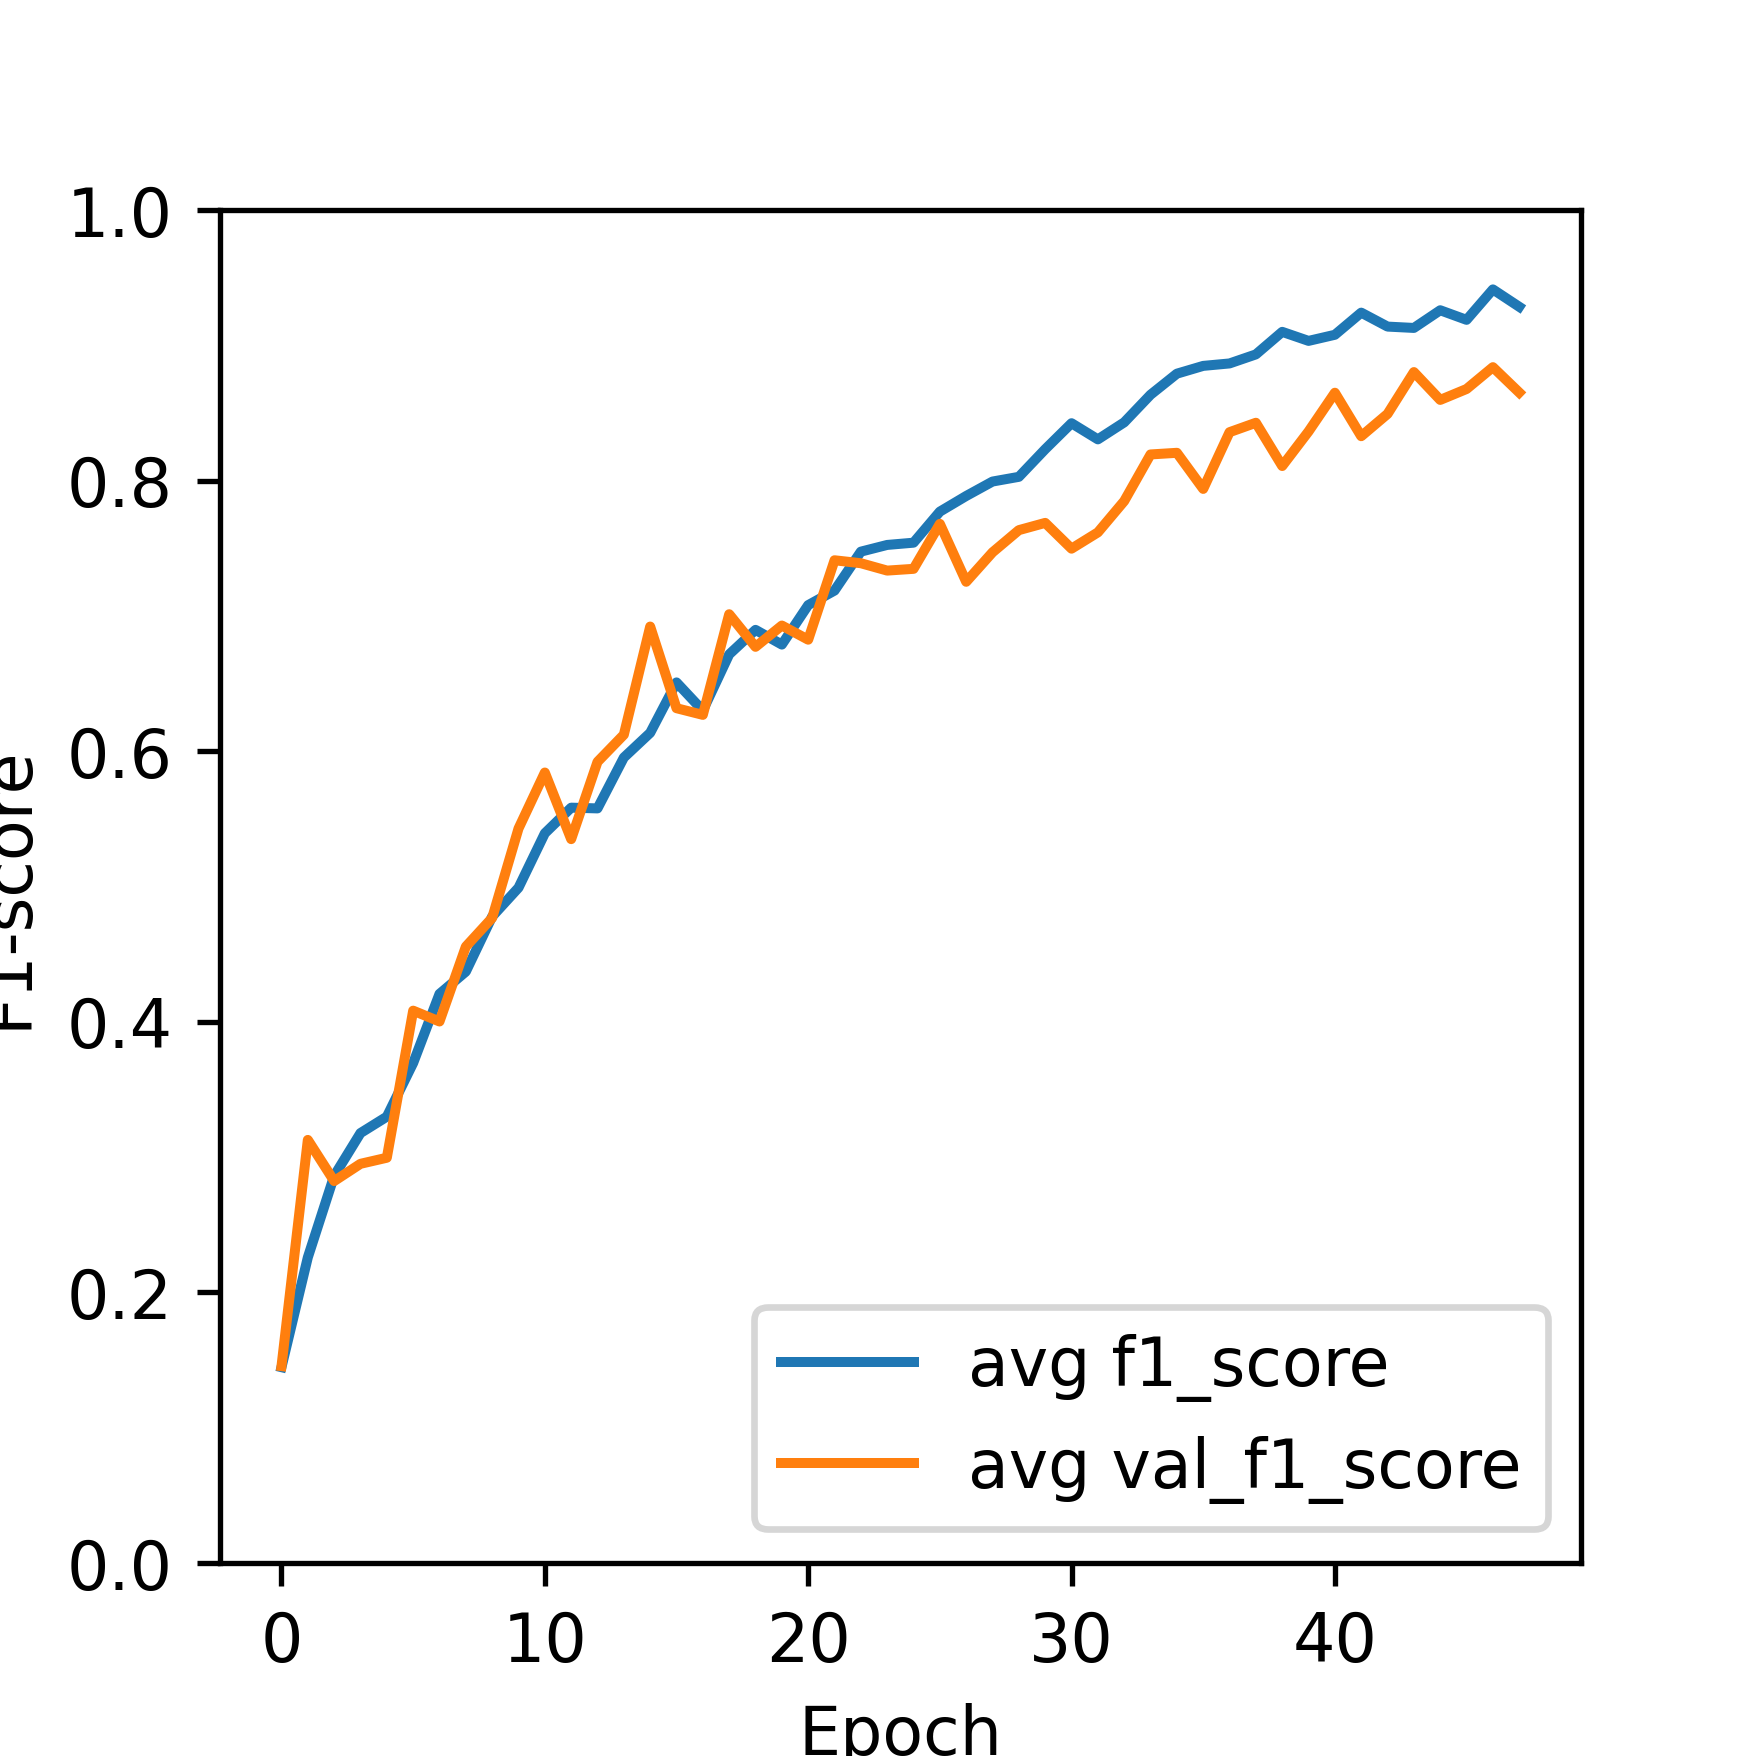
\includegraphics[width=.5\textwidth]{assets/results/preMELD.scratch/model.3dense/learning_history-f1_score.png}\hfill
	\caption{$F_1$ figures are from average from all $F_1^c$}
	\label{fig:figure6}
\end{figure}

\begin{figure}[H]
	\centering
	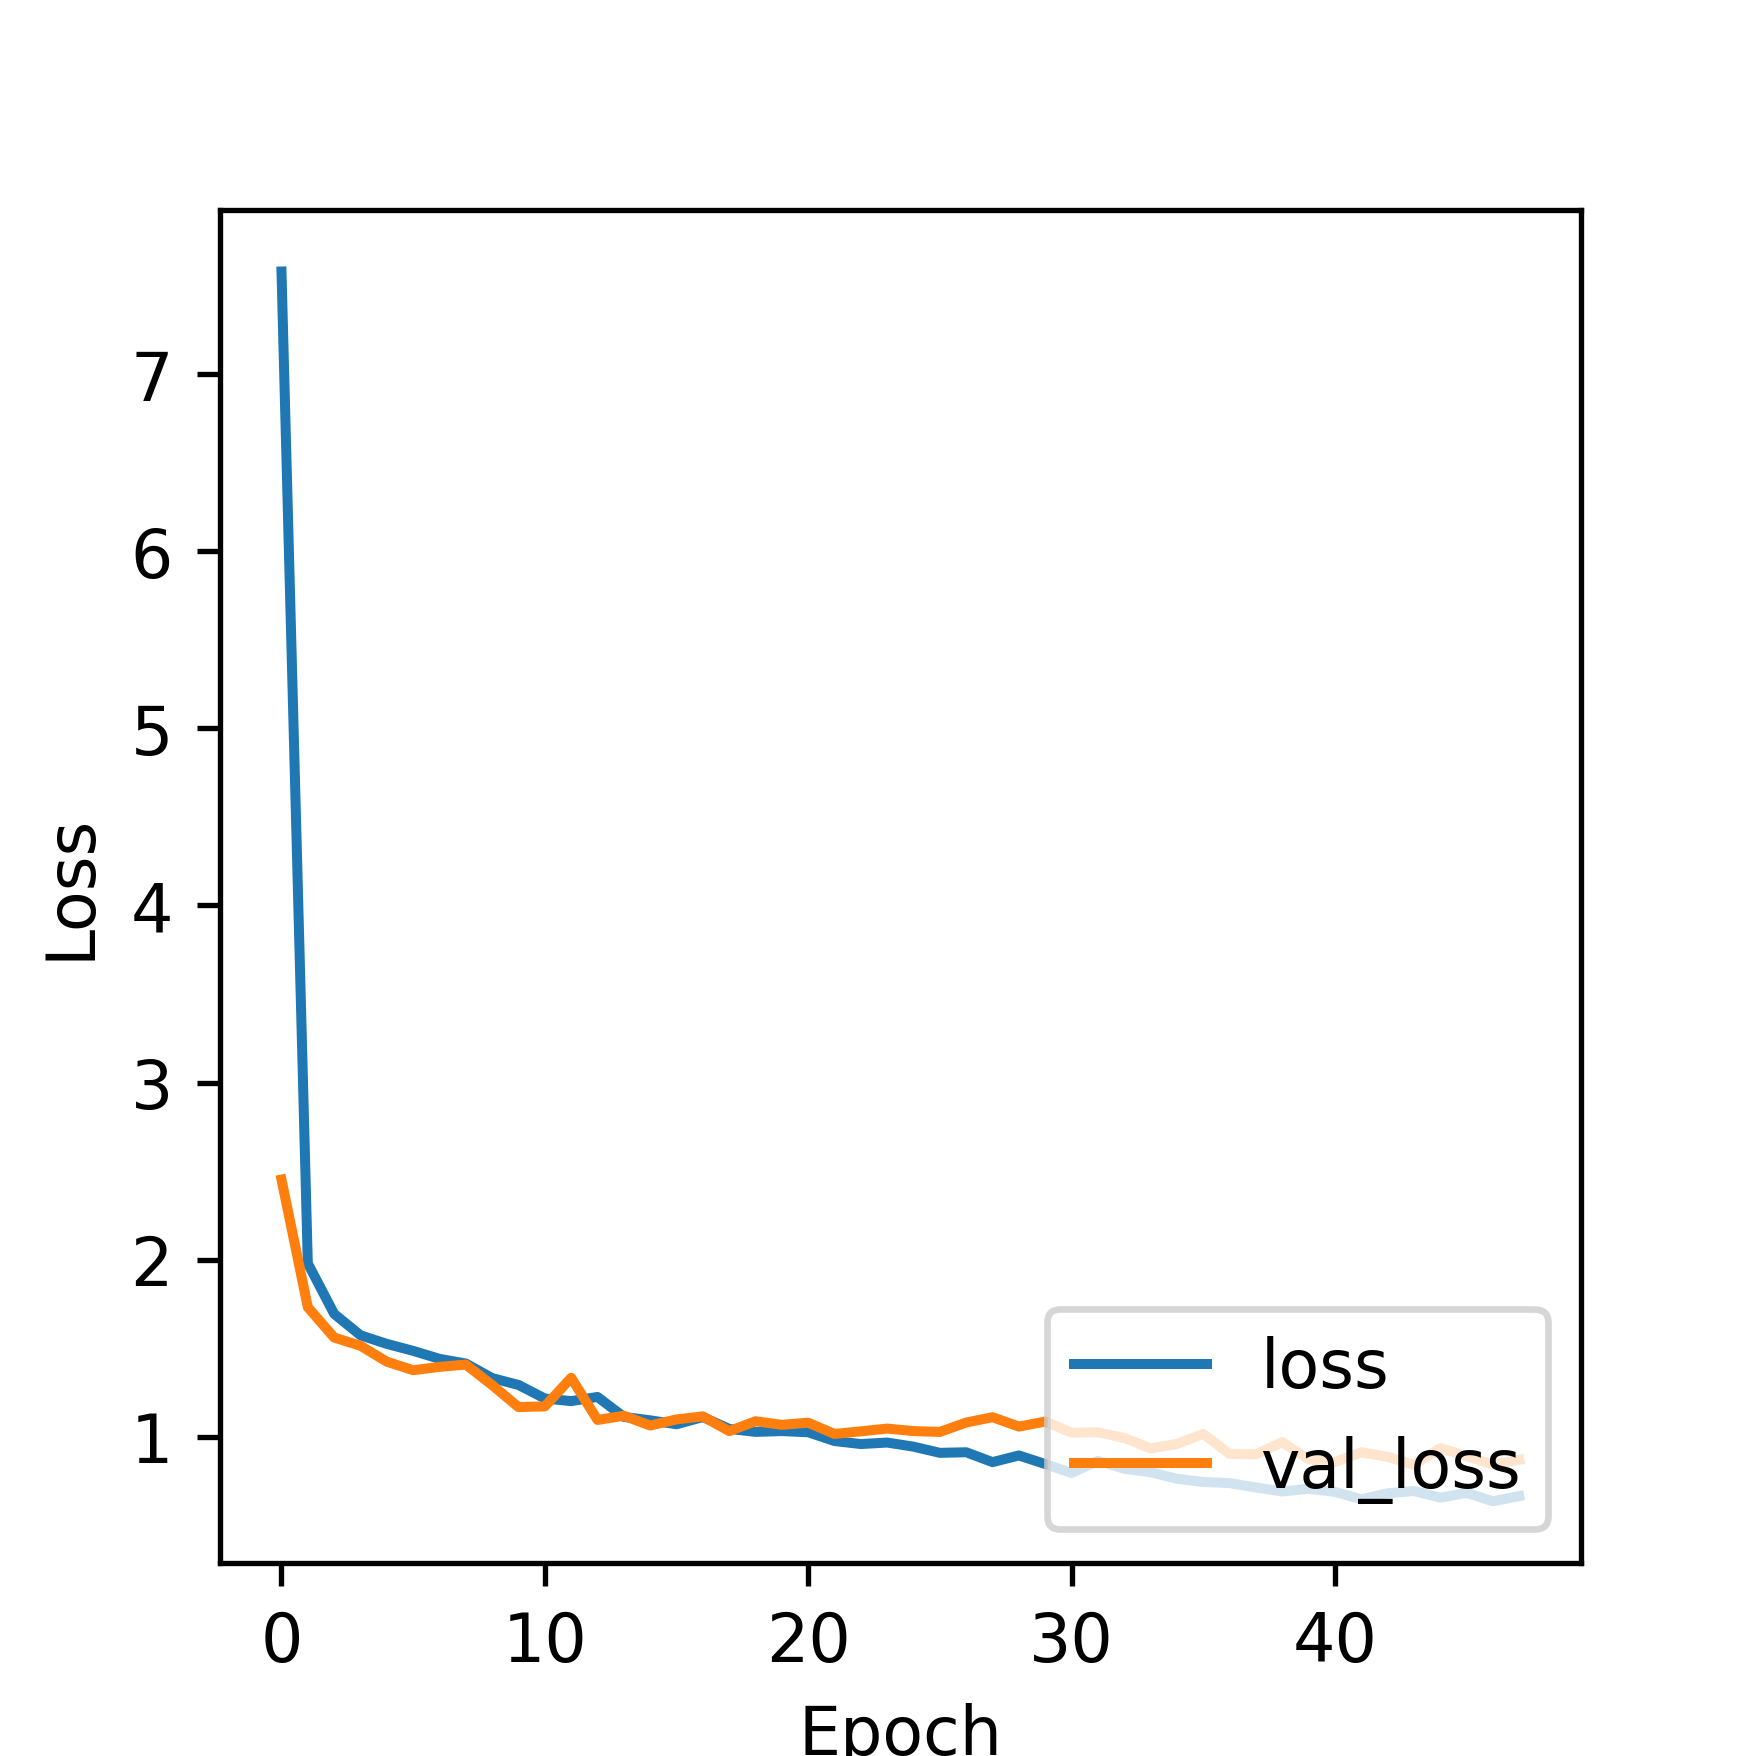
\includegraphics[width=.5\textwidth]{assets/results/preMELD.scratch/model.3dense/learning_history-loss.png}
	
	\label{fig:figure7}
\end{figure}

\begin{figure}[H]
	\centering
	\includegraphics[width=.95\textwidth]{assets/results/preMELD.scratch/model.3dense/confusion_matrix.png}
	
	\label{fig:cm3}
\end{figure}




\subsection{Data augmentation}

\paragraph{Architecture}
We tried to add augmentation to the two layers network \ref{scratch.2dense}. The architecture remains the same.

\lstinputlisting[language=Python,linerange={91-114}]{../train_scratch.py}

\paragraph{Augmentation}
We used a layer \texttt{tf.keras.layers.RandomContrast(0.5)} to adjust the spectrograms' contrasts during training

\paragraph{Results}
On the validation dataset, we obtained an accuracy $A_\text{val} = 0.64$ and the following $F_1$ scores:

\vspace{5mm}
\begin{tabular}{l|r}%
	\bfseries Class & \bfseries $F_1$% specify table head
	\csvreader[head to column names]{assets/results/preMELD.scratch/model.2dense.aug/f1.csv}{}% use head of csv as column names
	{\\\hline \class & \csvcolii}% specify your coloumns here
\end{tabular}
\vspace{5mm}

\begin{figure}[H]
	\centering
	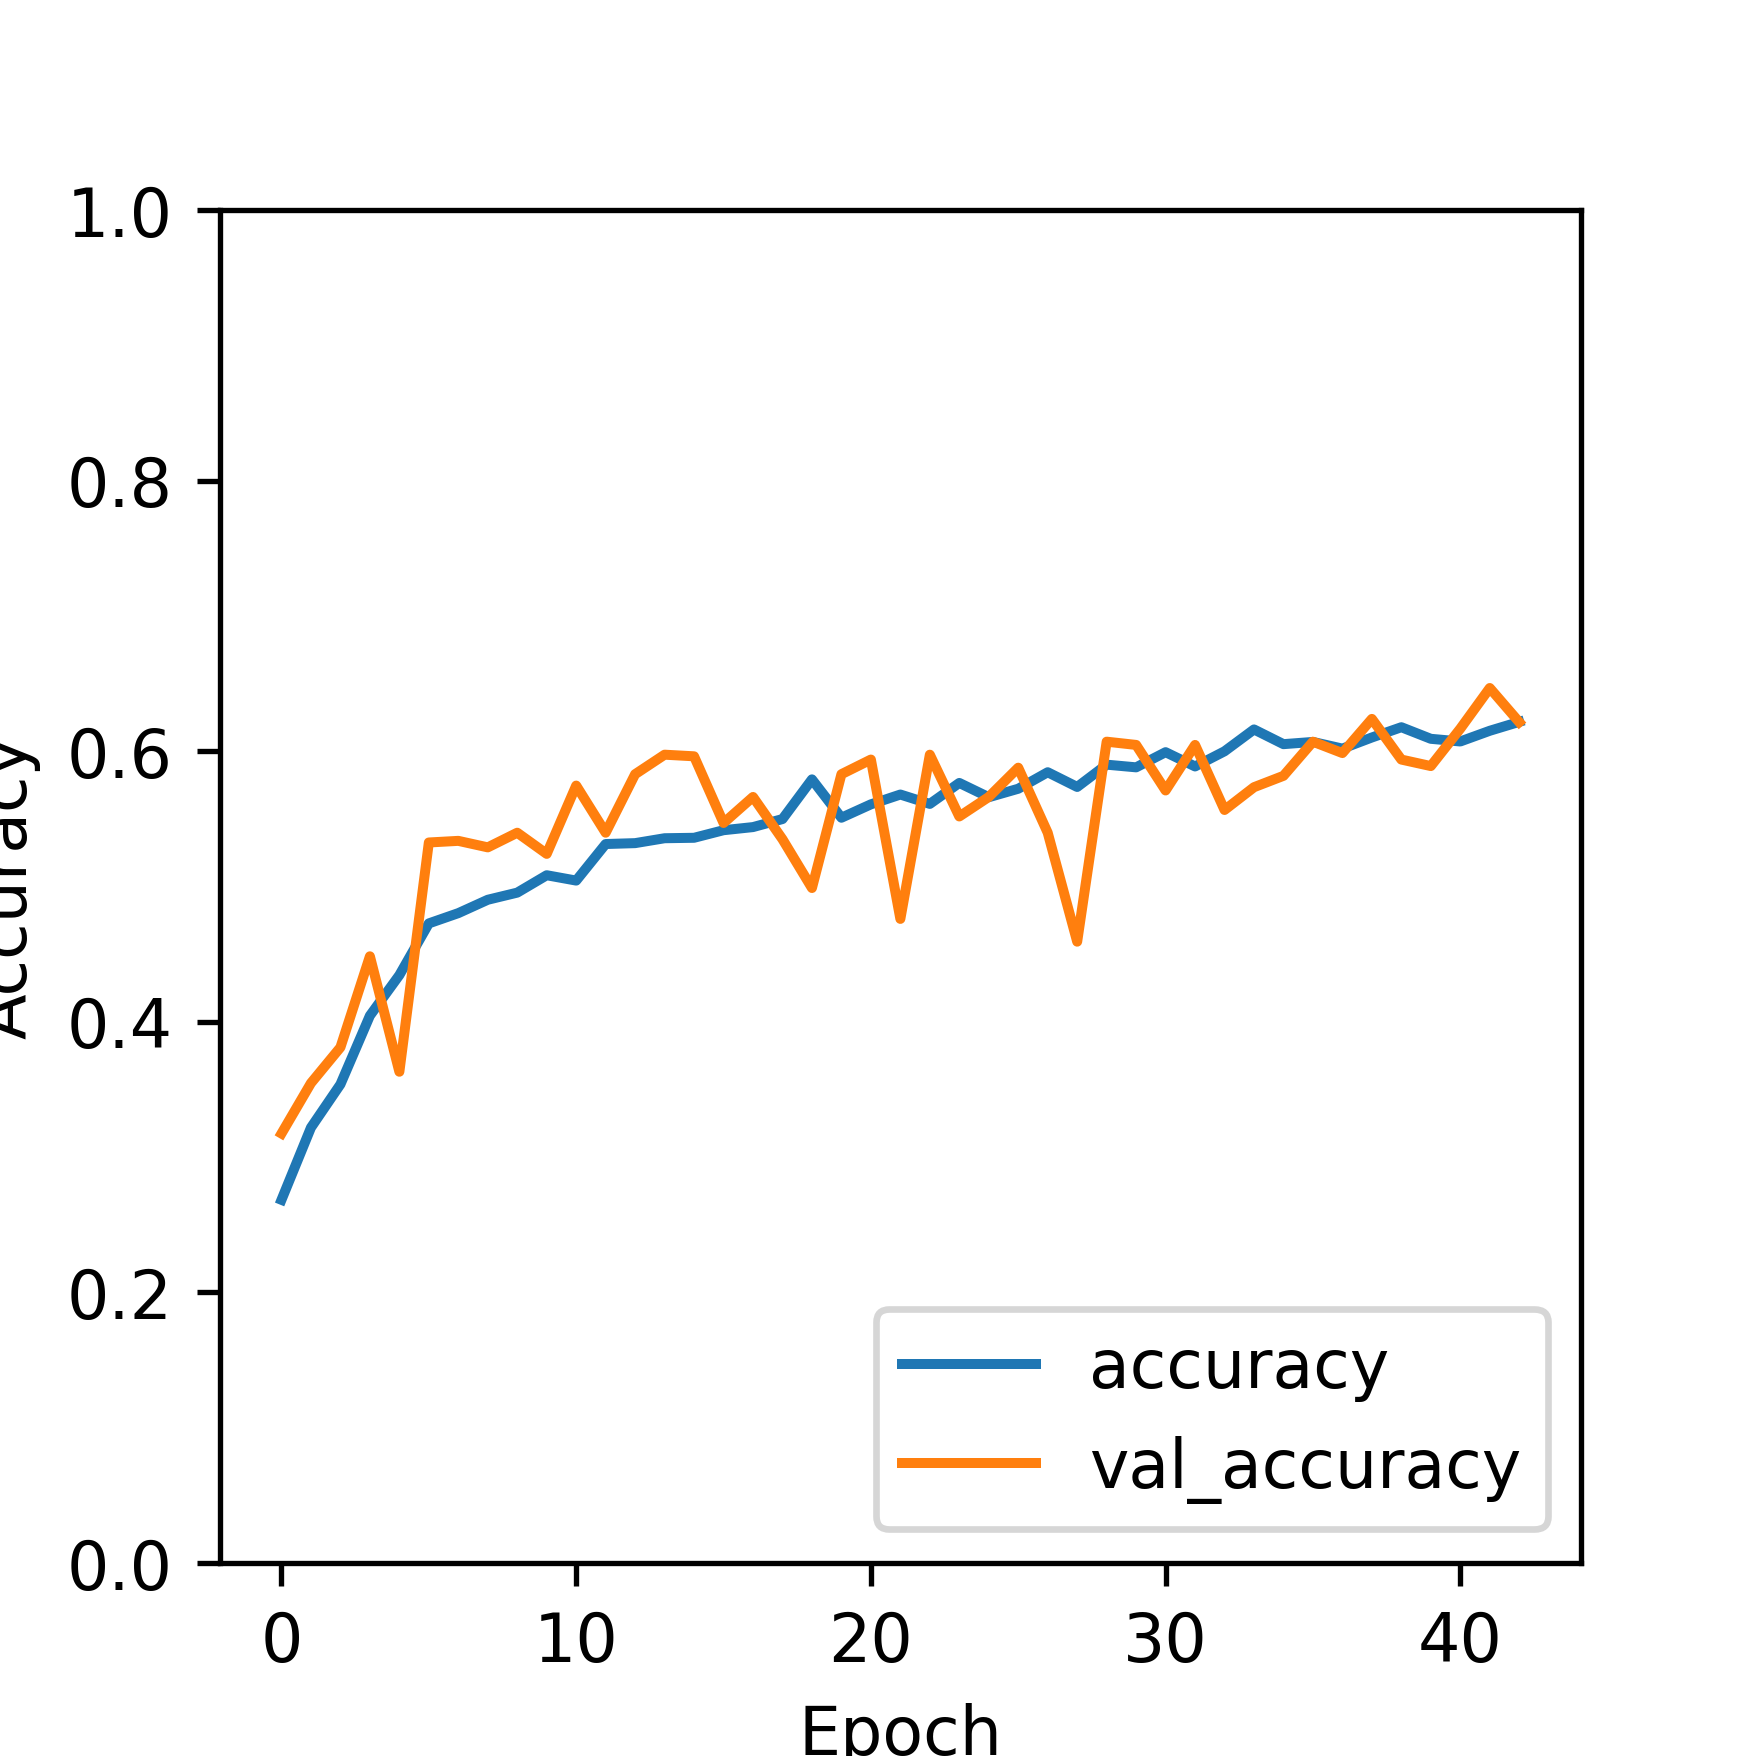
\includegraphics[width=.5\textwidth]{assets/results/preMELD.scratch/model.2dense.aug/learning_history-acc.png}\hfill
	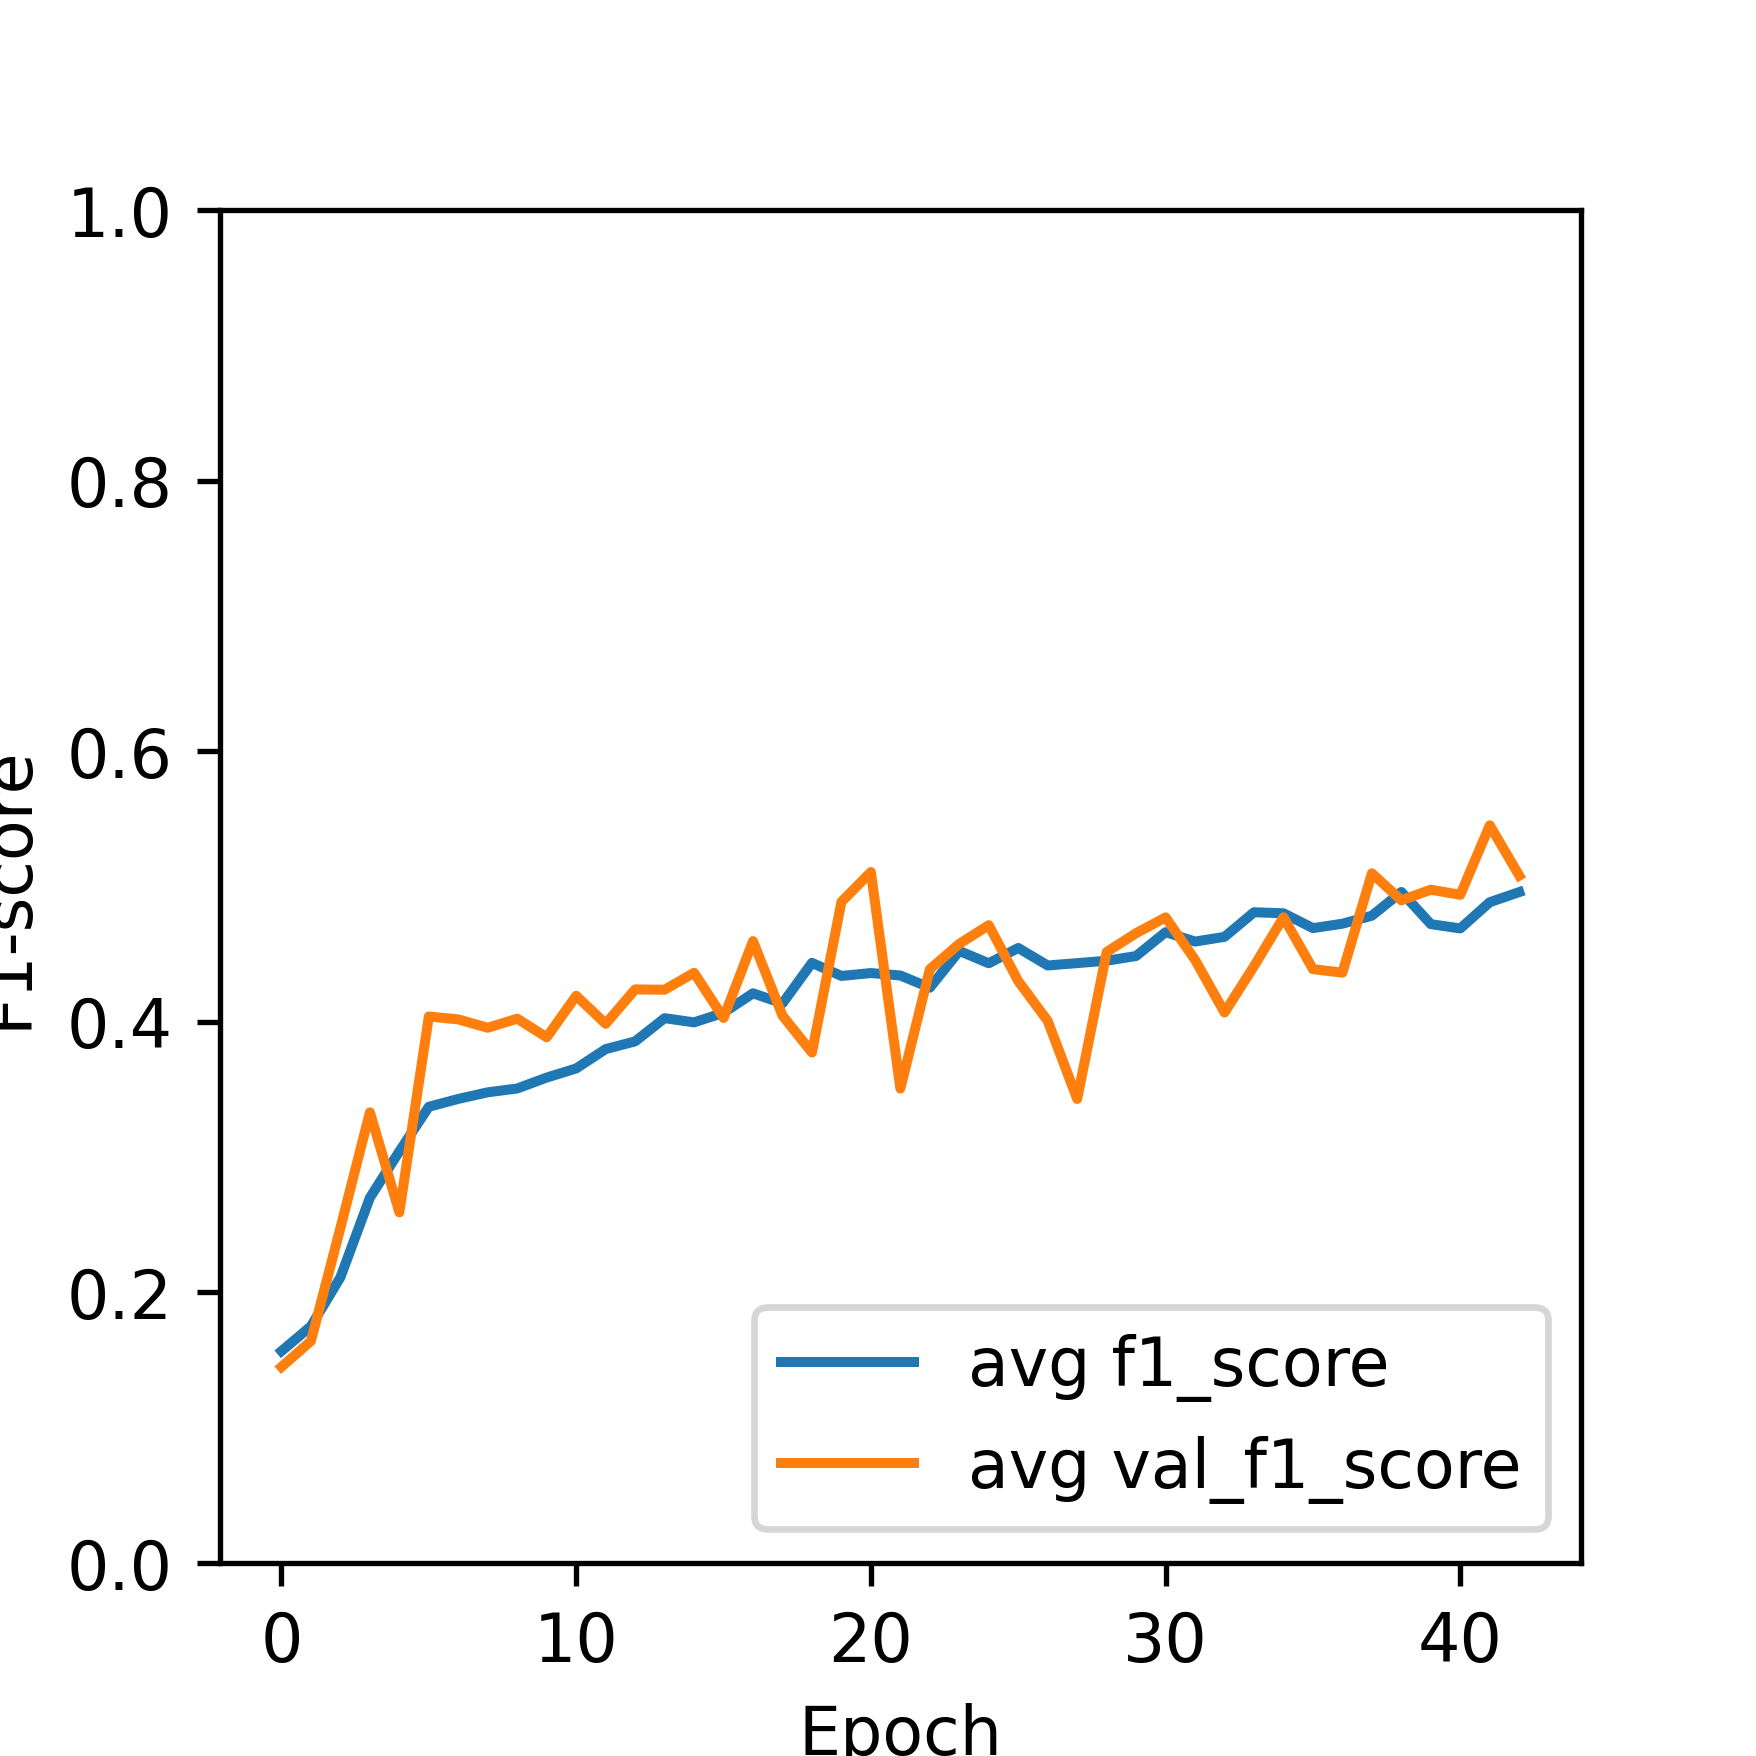
\includegraphics[width=.5\textwidth]{assets/results/preMELD.scratch/model.2dense.aug/learning_history-f1_score.png}\hfill
	\caption{$F_1$ figures are from average from all $F_1^c$}
	\label{fig:figure8}
\end{figure}

\begin{figure}[H]
	\centering
	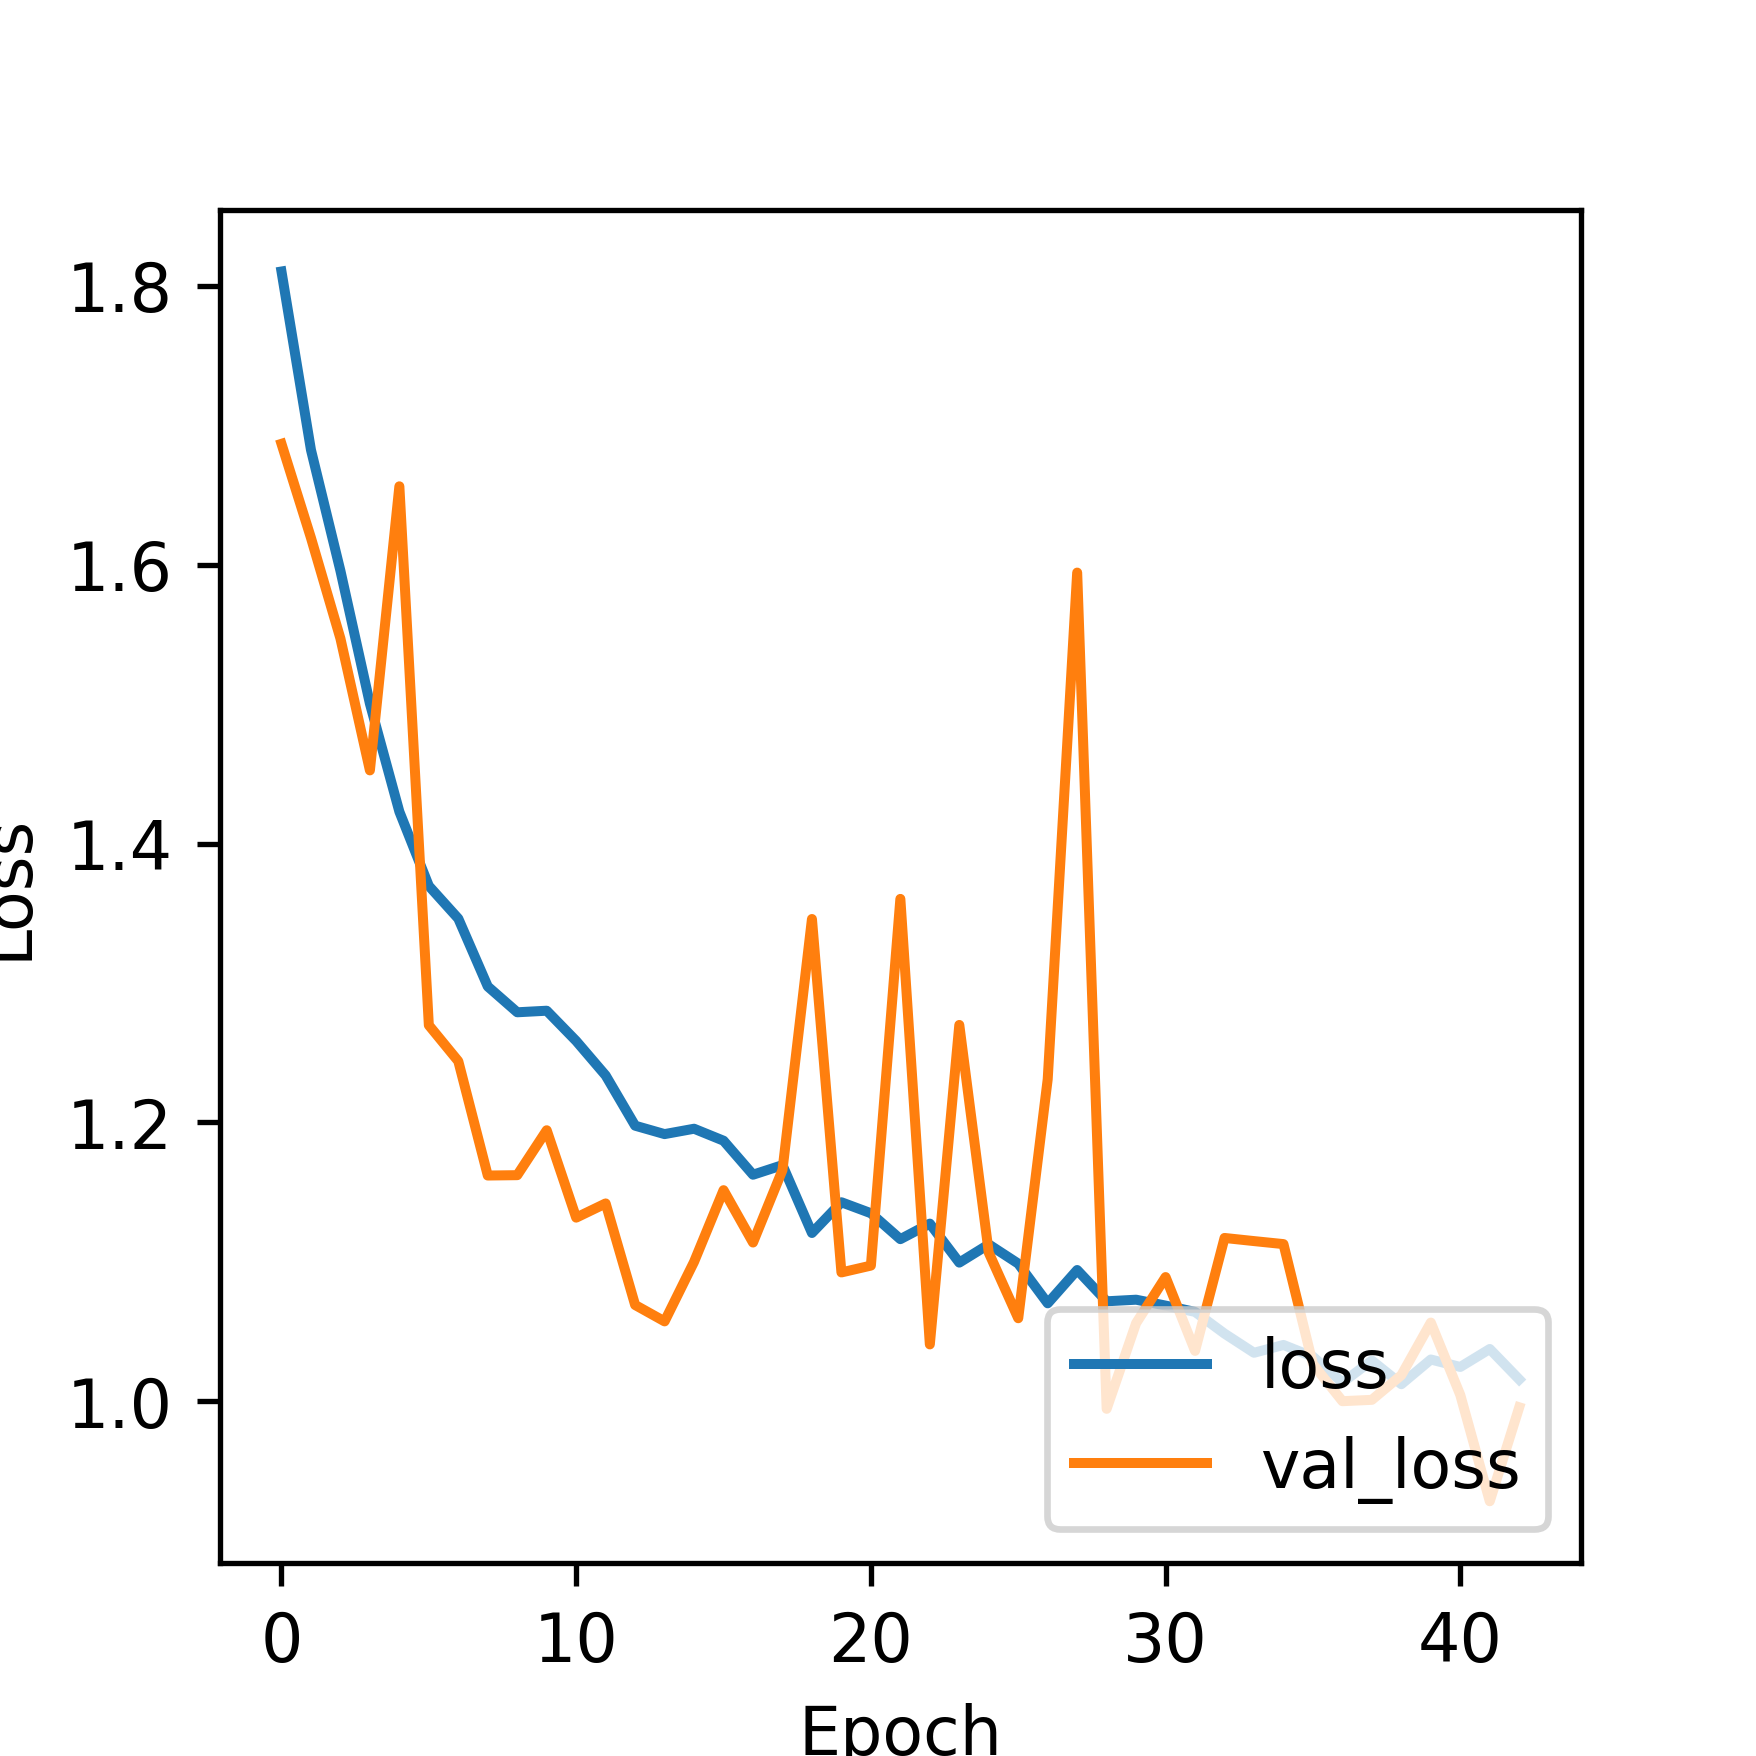
\includegraphics[width=.5\textwidth]{assets/results/preMELD.scratch/model.2dense.aug/learning_history-loss.png}
	
	\label{fig:figure9}
\end{figure}

\paragraph{}
From the confusion matrix we can see how this model tends to choose the majority class.

\begin{figure}[H]
	\centering
	\includegraphics[width=.95\textwidth]{assets/results/preMELD.scratch/model.2dense.aug/confusion_matrix.png}
	
	\label{fig:cm4}
\end{figure}







\section{Pre-trained models}

\paragraph{Model}
We chosed \emph{VGG16} as our pre-trained model. It's to be noted that all those pre-trained models were trained on real photographs, so we didn't expect good results since they never saw a picture of a MEL spectrogram; nevertheless we tried anyway and the result were not as bad as we initially thought.

\subsection{Feature extraction from VGG16}

\paragraph{Architecture}

\lstinputlisting[language=Python,linerange={85-95}]{../fine_tuning.py}


\paragraph{Results}
On the validation dataset, we obtained an accuracy $A_\text{val} = 0.75$ and the following $F_1$ scores:

\vspace{5mm}
\begin{tabular}{l|r}%
	\bfseries Class & \bfseries $F_1$% specify table head
	\csvreader[head to column names]{assets/results/preMELD.vgg/vgg16_feature_extract/f1.csv}{}% use head of csv as column names
	{\\\hline \class & \csvcolii}% specify your coloumns here
\end{tabular}
\vspace{5mm}

\begin{figure}[H]
	\centering
	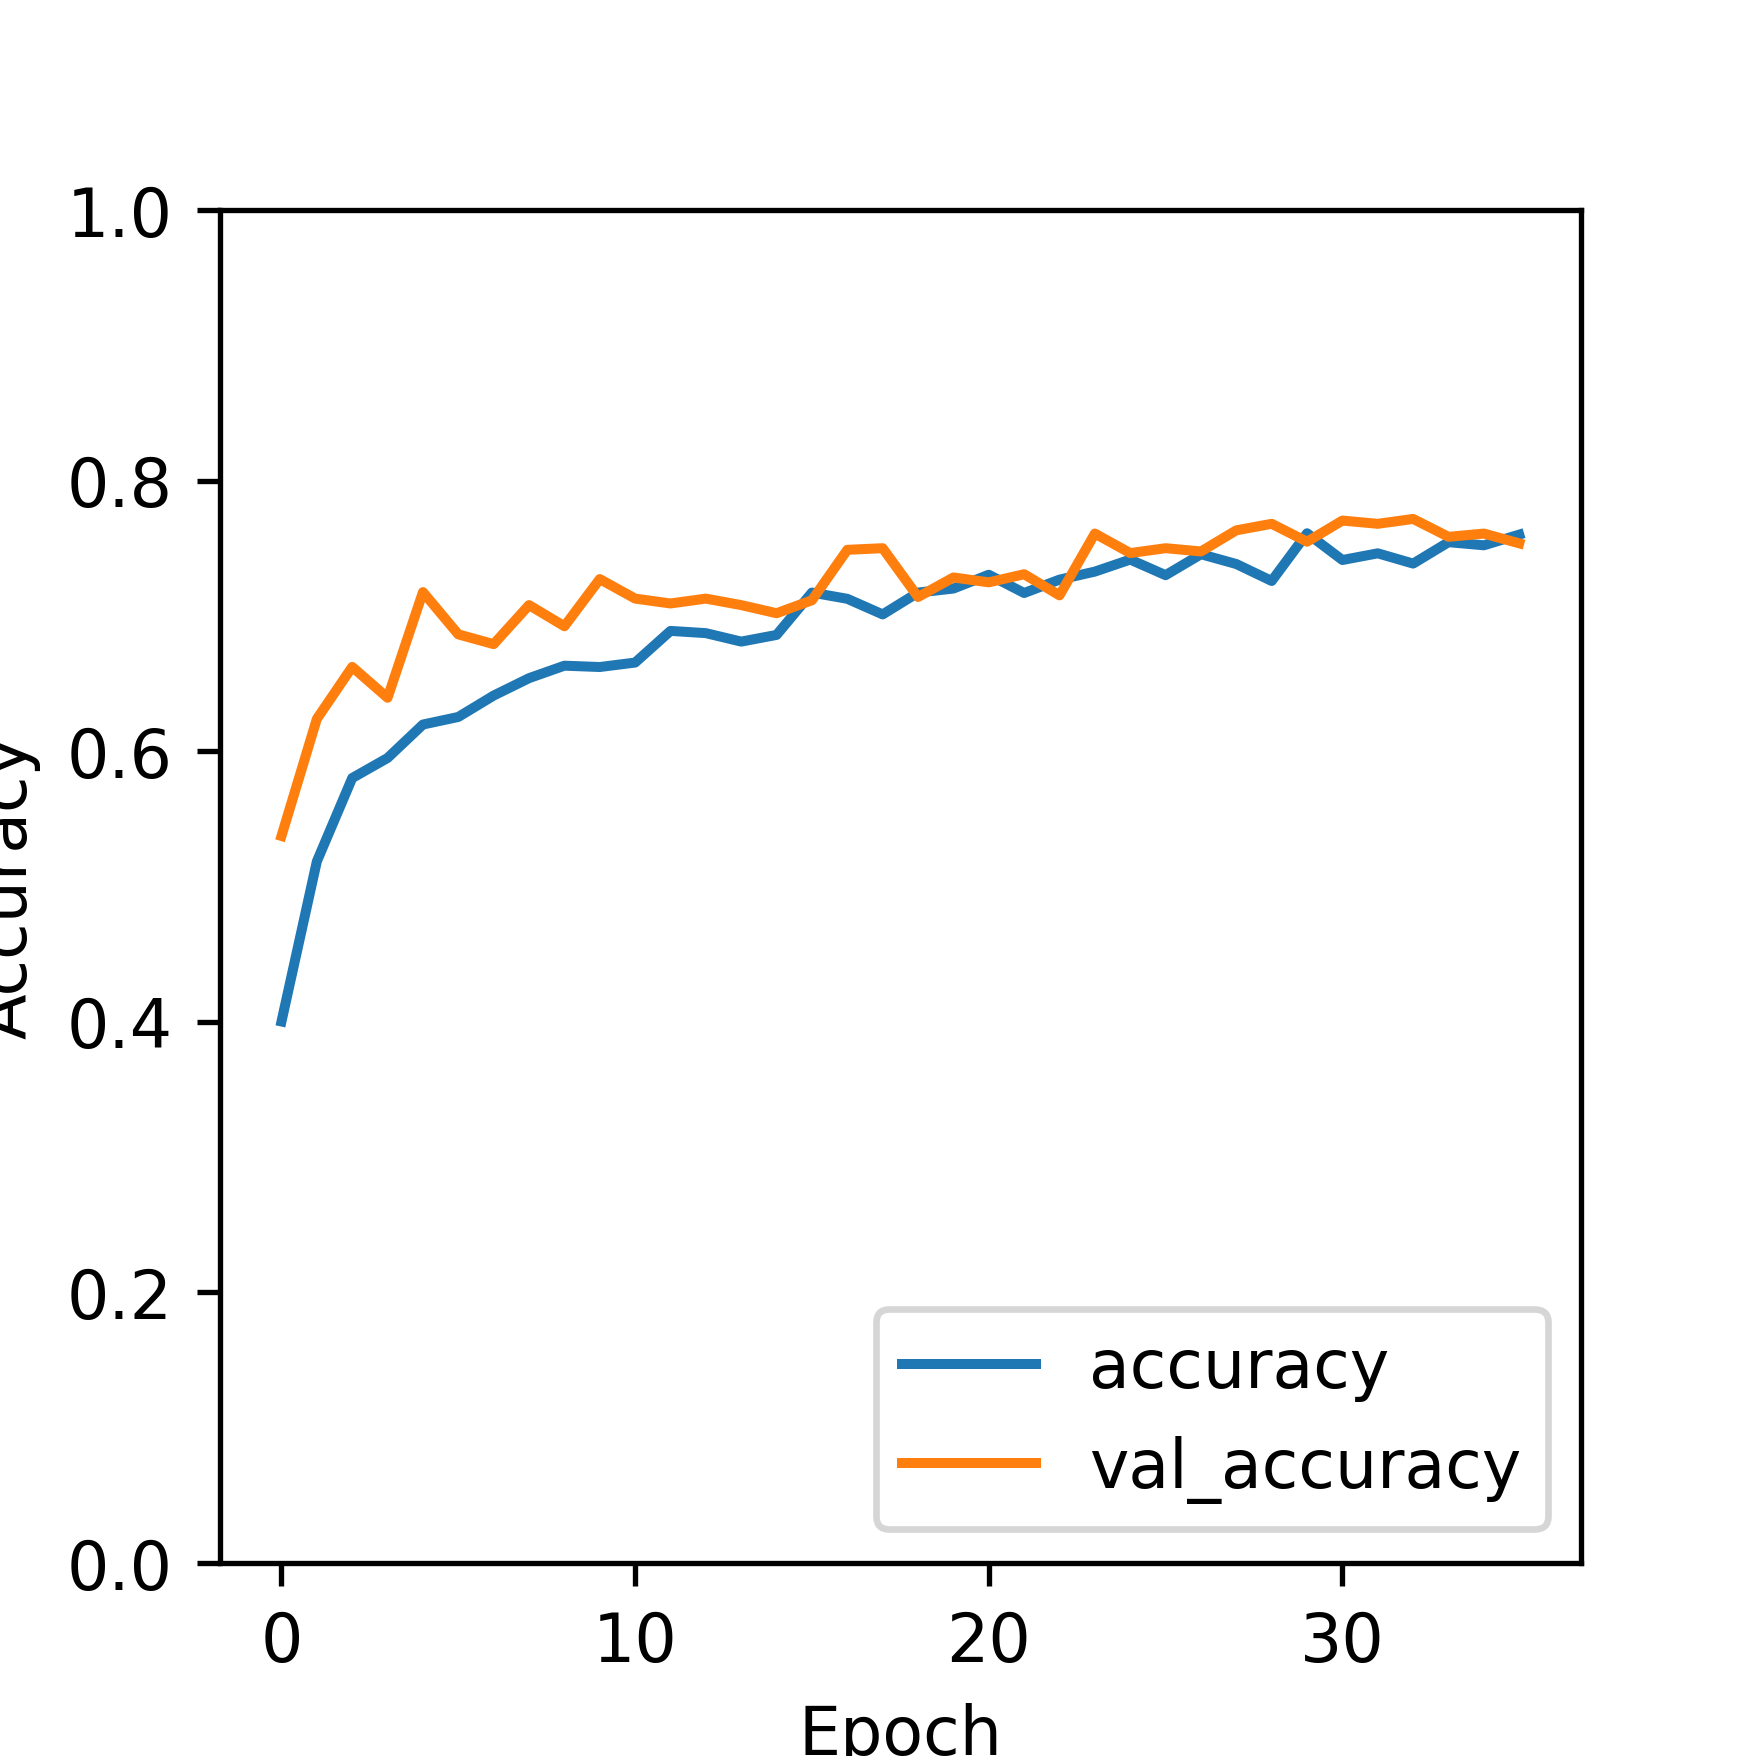
\includegraphics[width=.5\textwidth]{assets/results/preMELD.vgg/vgg16_feature_extract/learning_history-acc.png}\hfill
	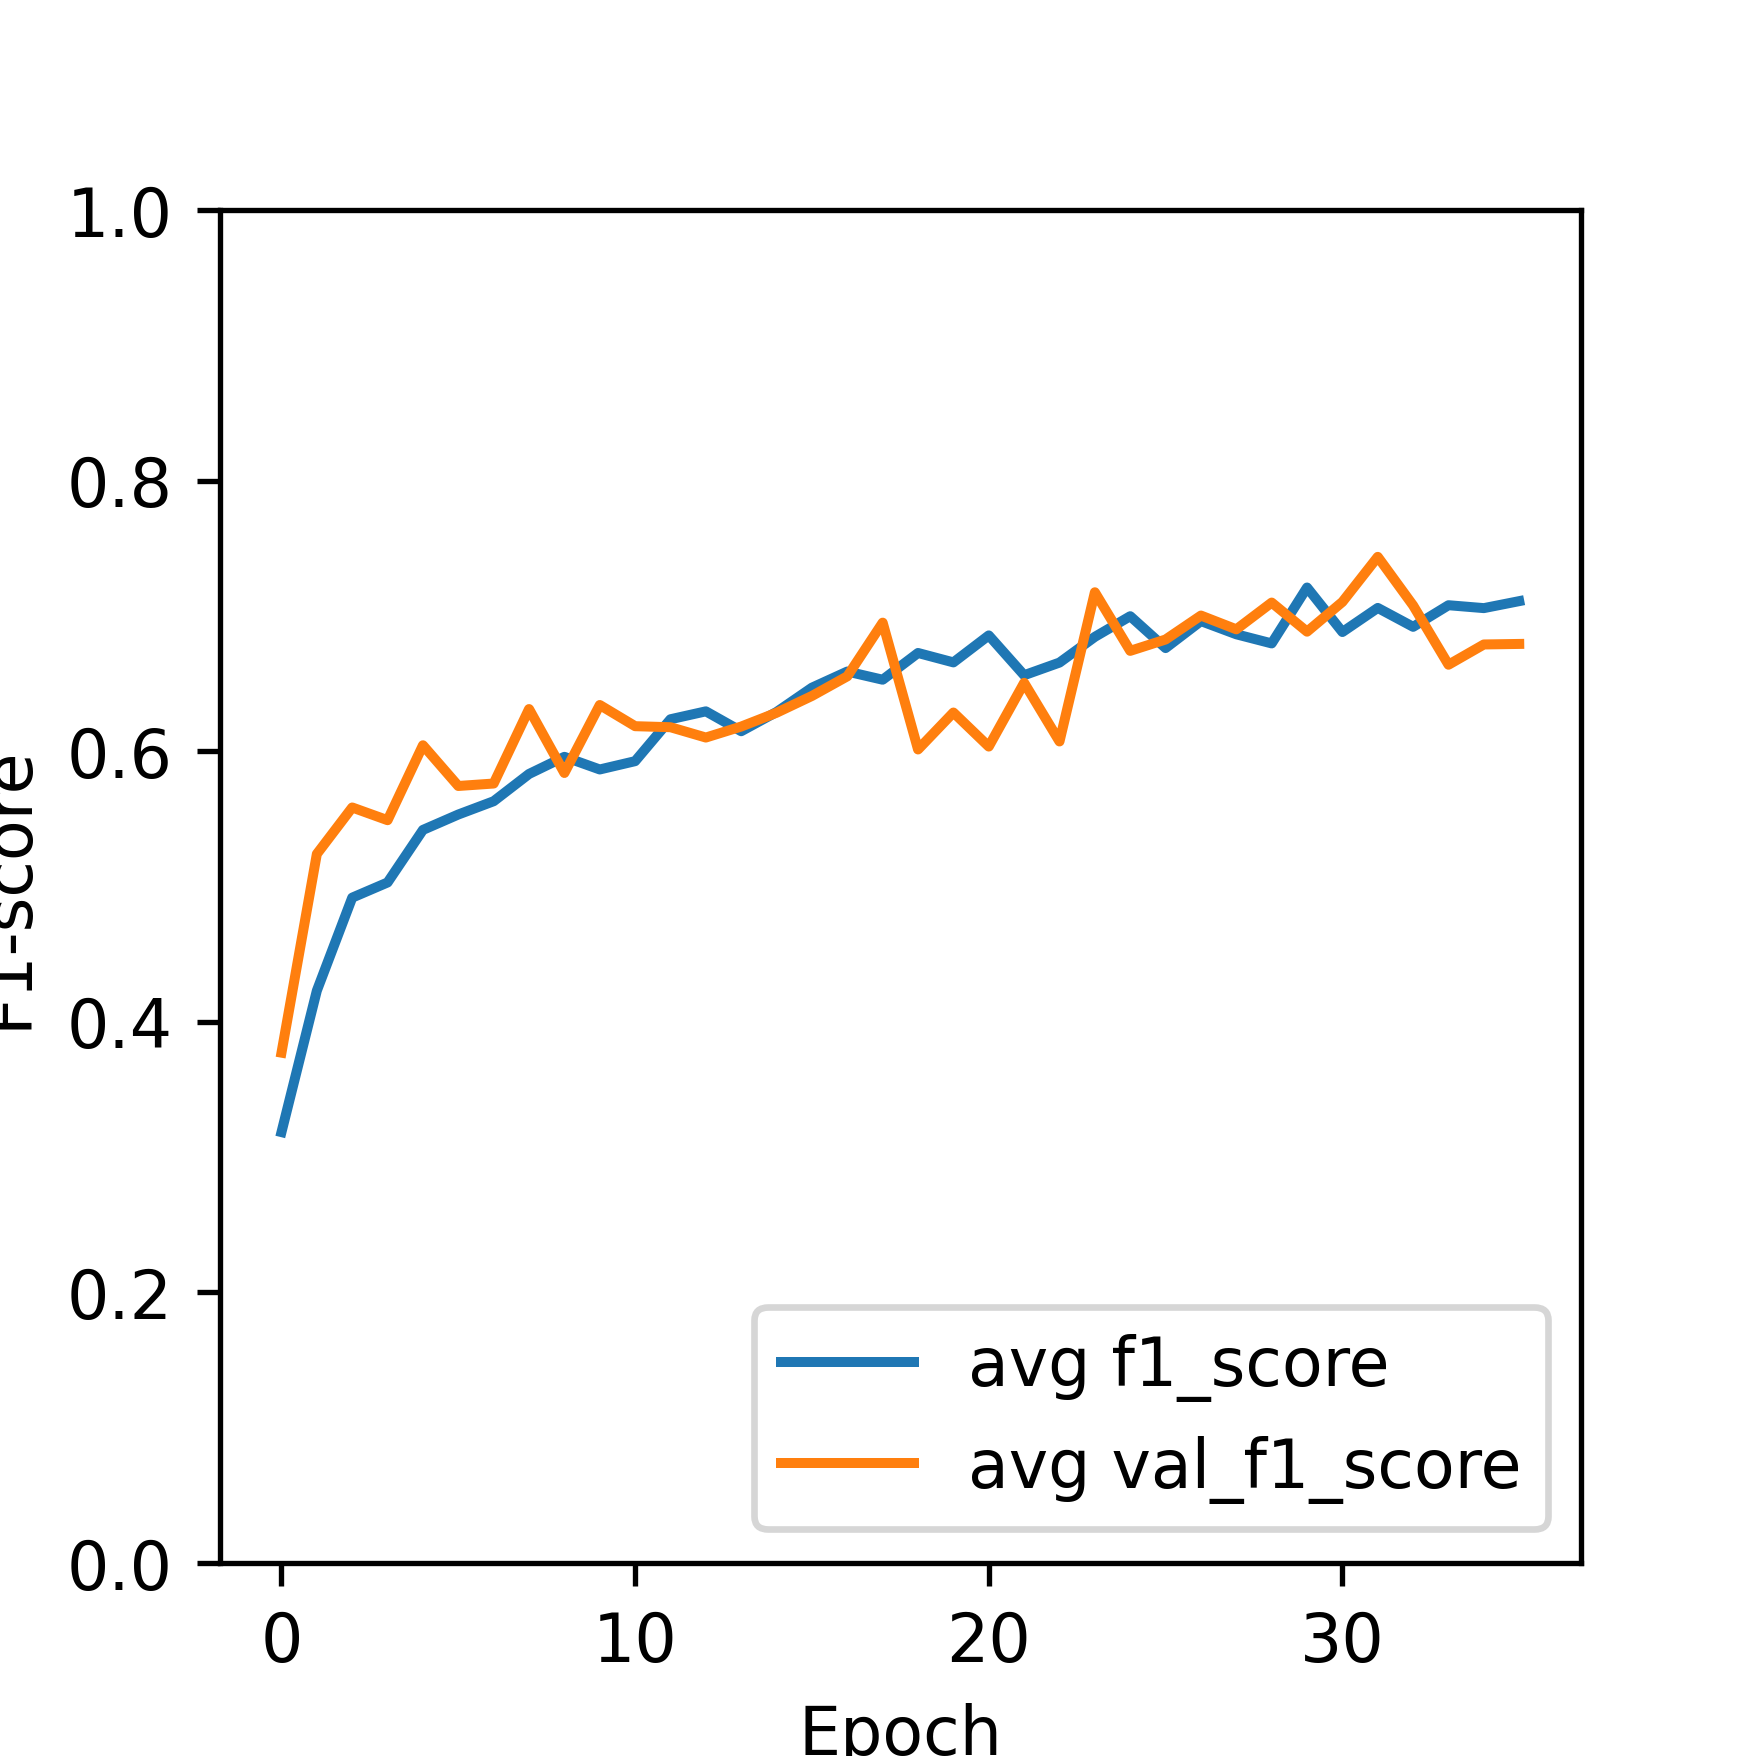
\includegraphics[width=.5\textwidth]{assets/results/preMELD.vgg/vgg16_feature_extract/learning_history-f1_score.png}\hfill
	\caption{$F_1$ figures are from average from all $F_1^c$}
	\label{fig:figure10}
\end{figure}

\begin{figure}[H]
	\centering
	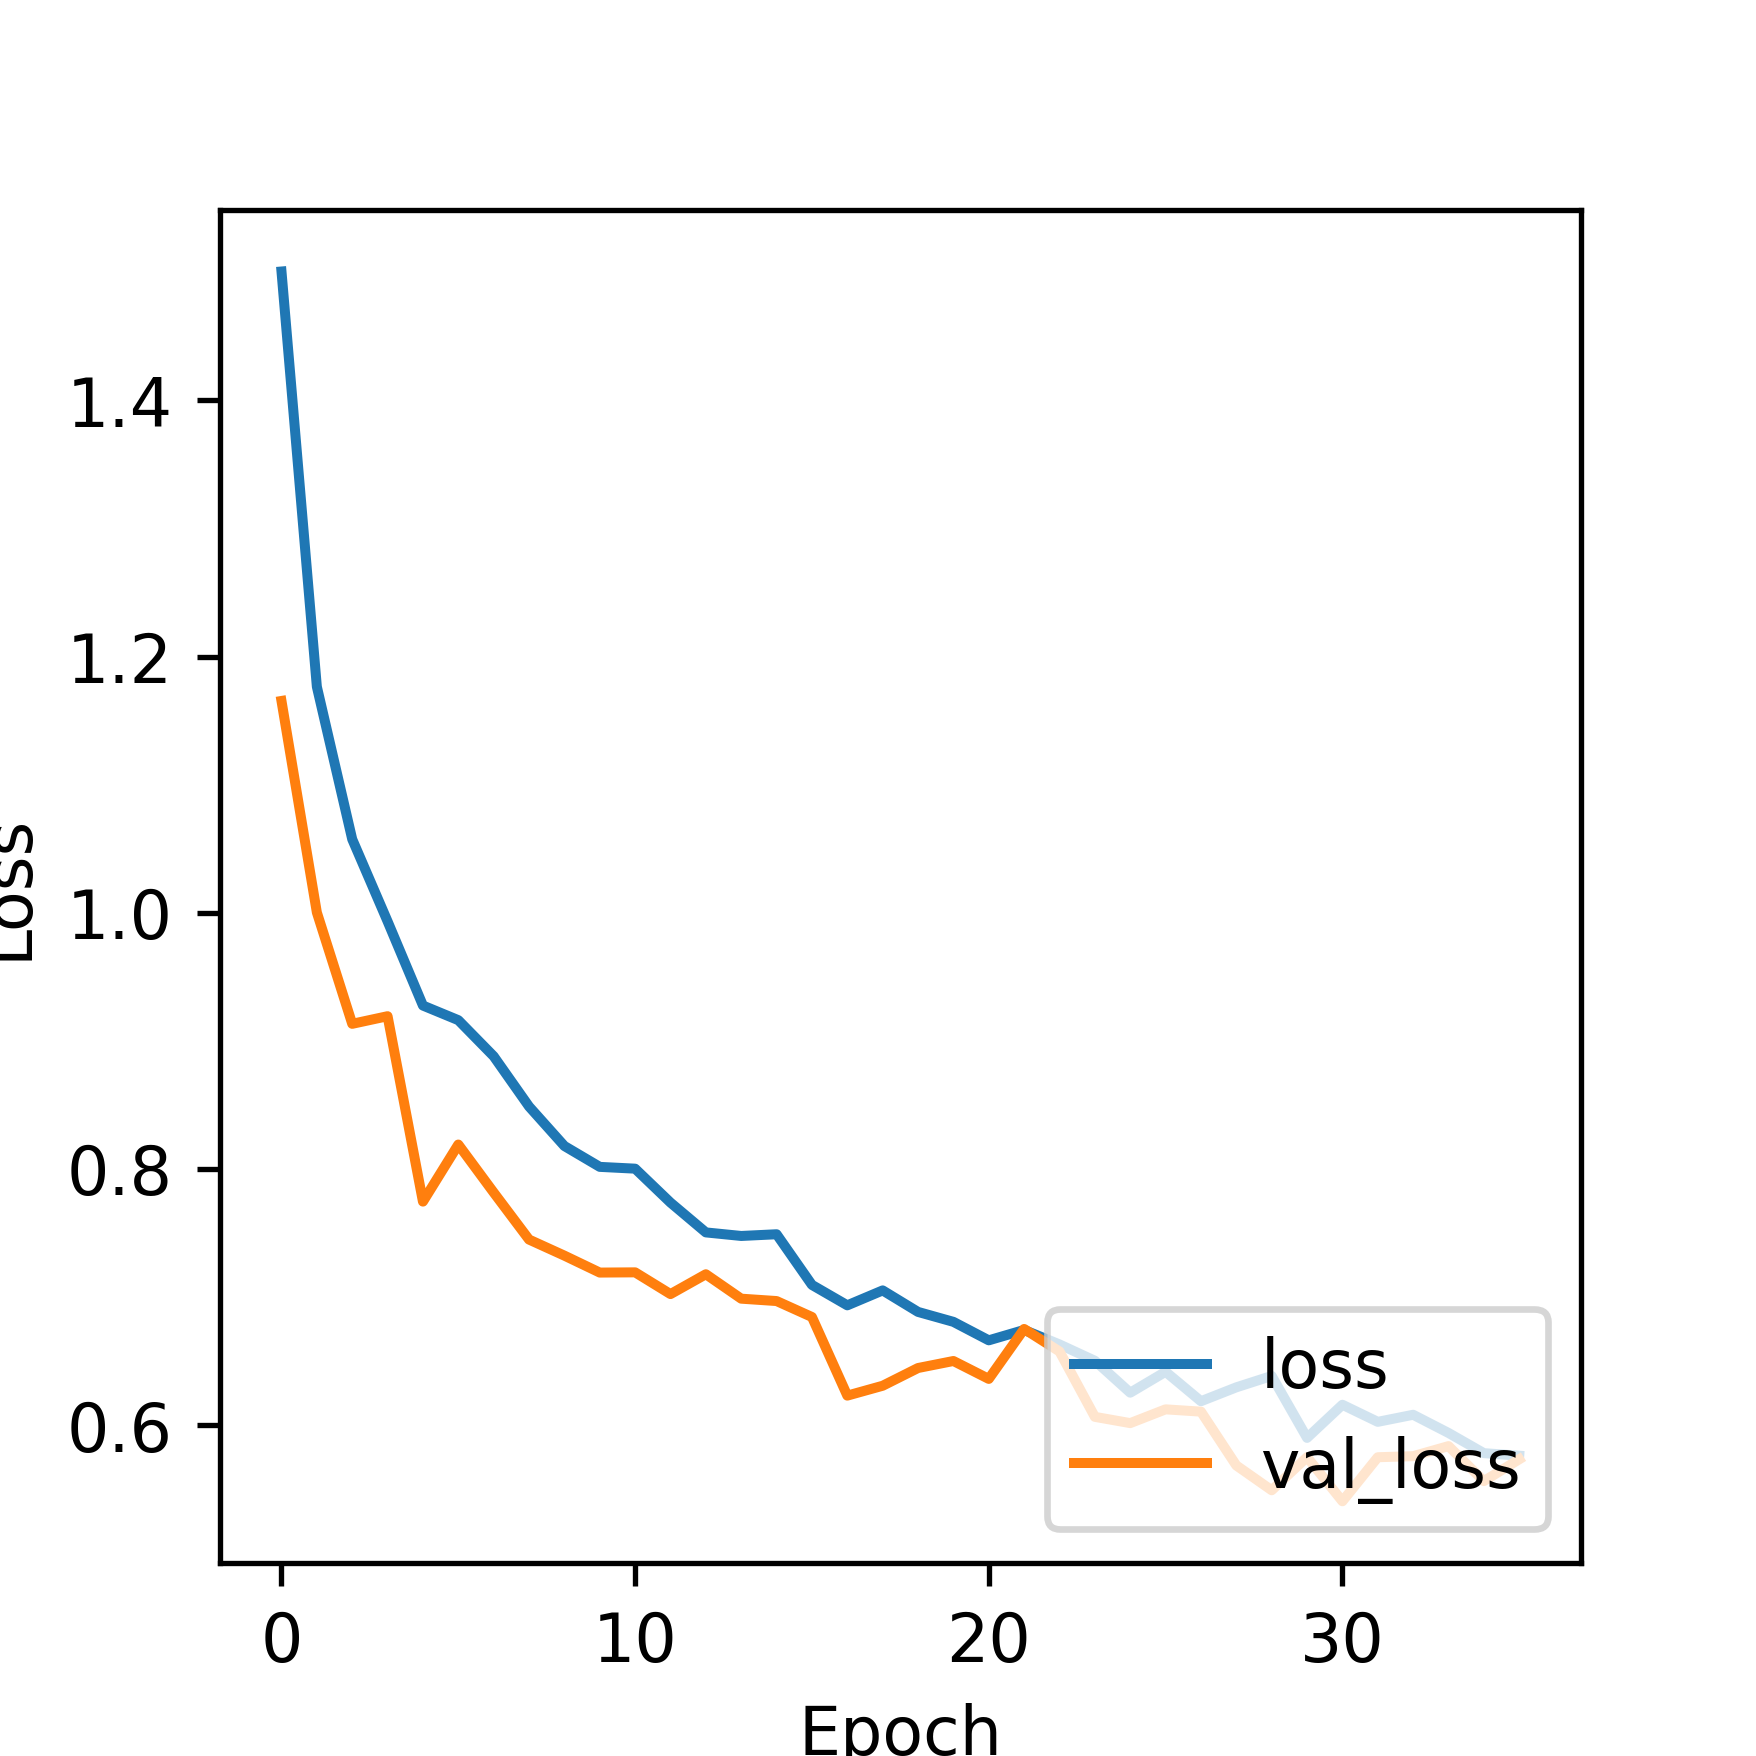
\includegraphics[width=.5\textwidth]{assets/results/preMELD.vgg/vgg16_feature_extract/learning_history-loss.png}
	
	\label{fig:figure13}
\end{figure}

\begin{figure}[H]
	\centering
	\includegraphics[width=.95\textwidth]{assets/results/preMELD.vgg/vgg16_feature_extract/confusion_matrix.png}
	
	\label{fig:cm6}
\end{figure}





\subsection{Fine tuning with VGG16}

\paragraph{Architecture}

The same as before but some layers were un-freeze.

\lstinputlisting[language=Python,linerange={112-119}]{../fine_tuning.py}


\paragraph{Results}
On the validation dataset, we obtained an accuracy $A_\text{val} = 0.25$ and the following $F_1$ scores:

\vspace{5mm}
\begin{tabular}{l|r}%
	\bfseries Class & \bfseries $F_1$% specify table head
	\csvreader[head to column names]{assets/results/preMELD.vgg/vgg16_finetune/f1.csv}{}% use head of csv as column names
	{\\\hline \class & \csvcolii}% specify your coloumns here
\end{tabular}
\vspace{5mm}

\begin{figure}[H]
	\centering
	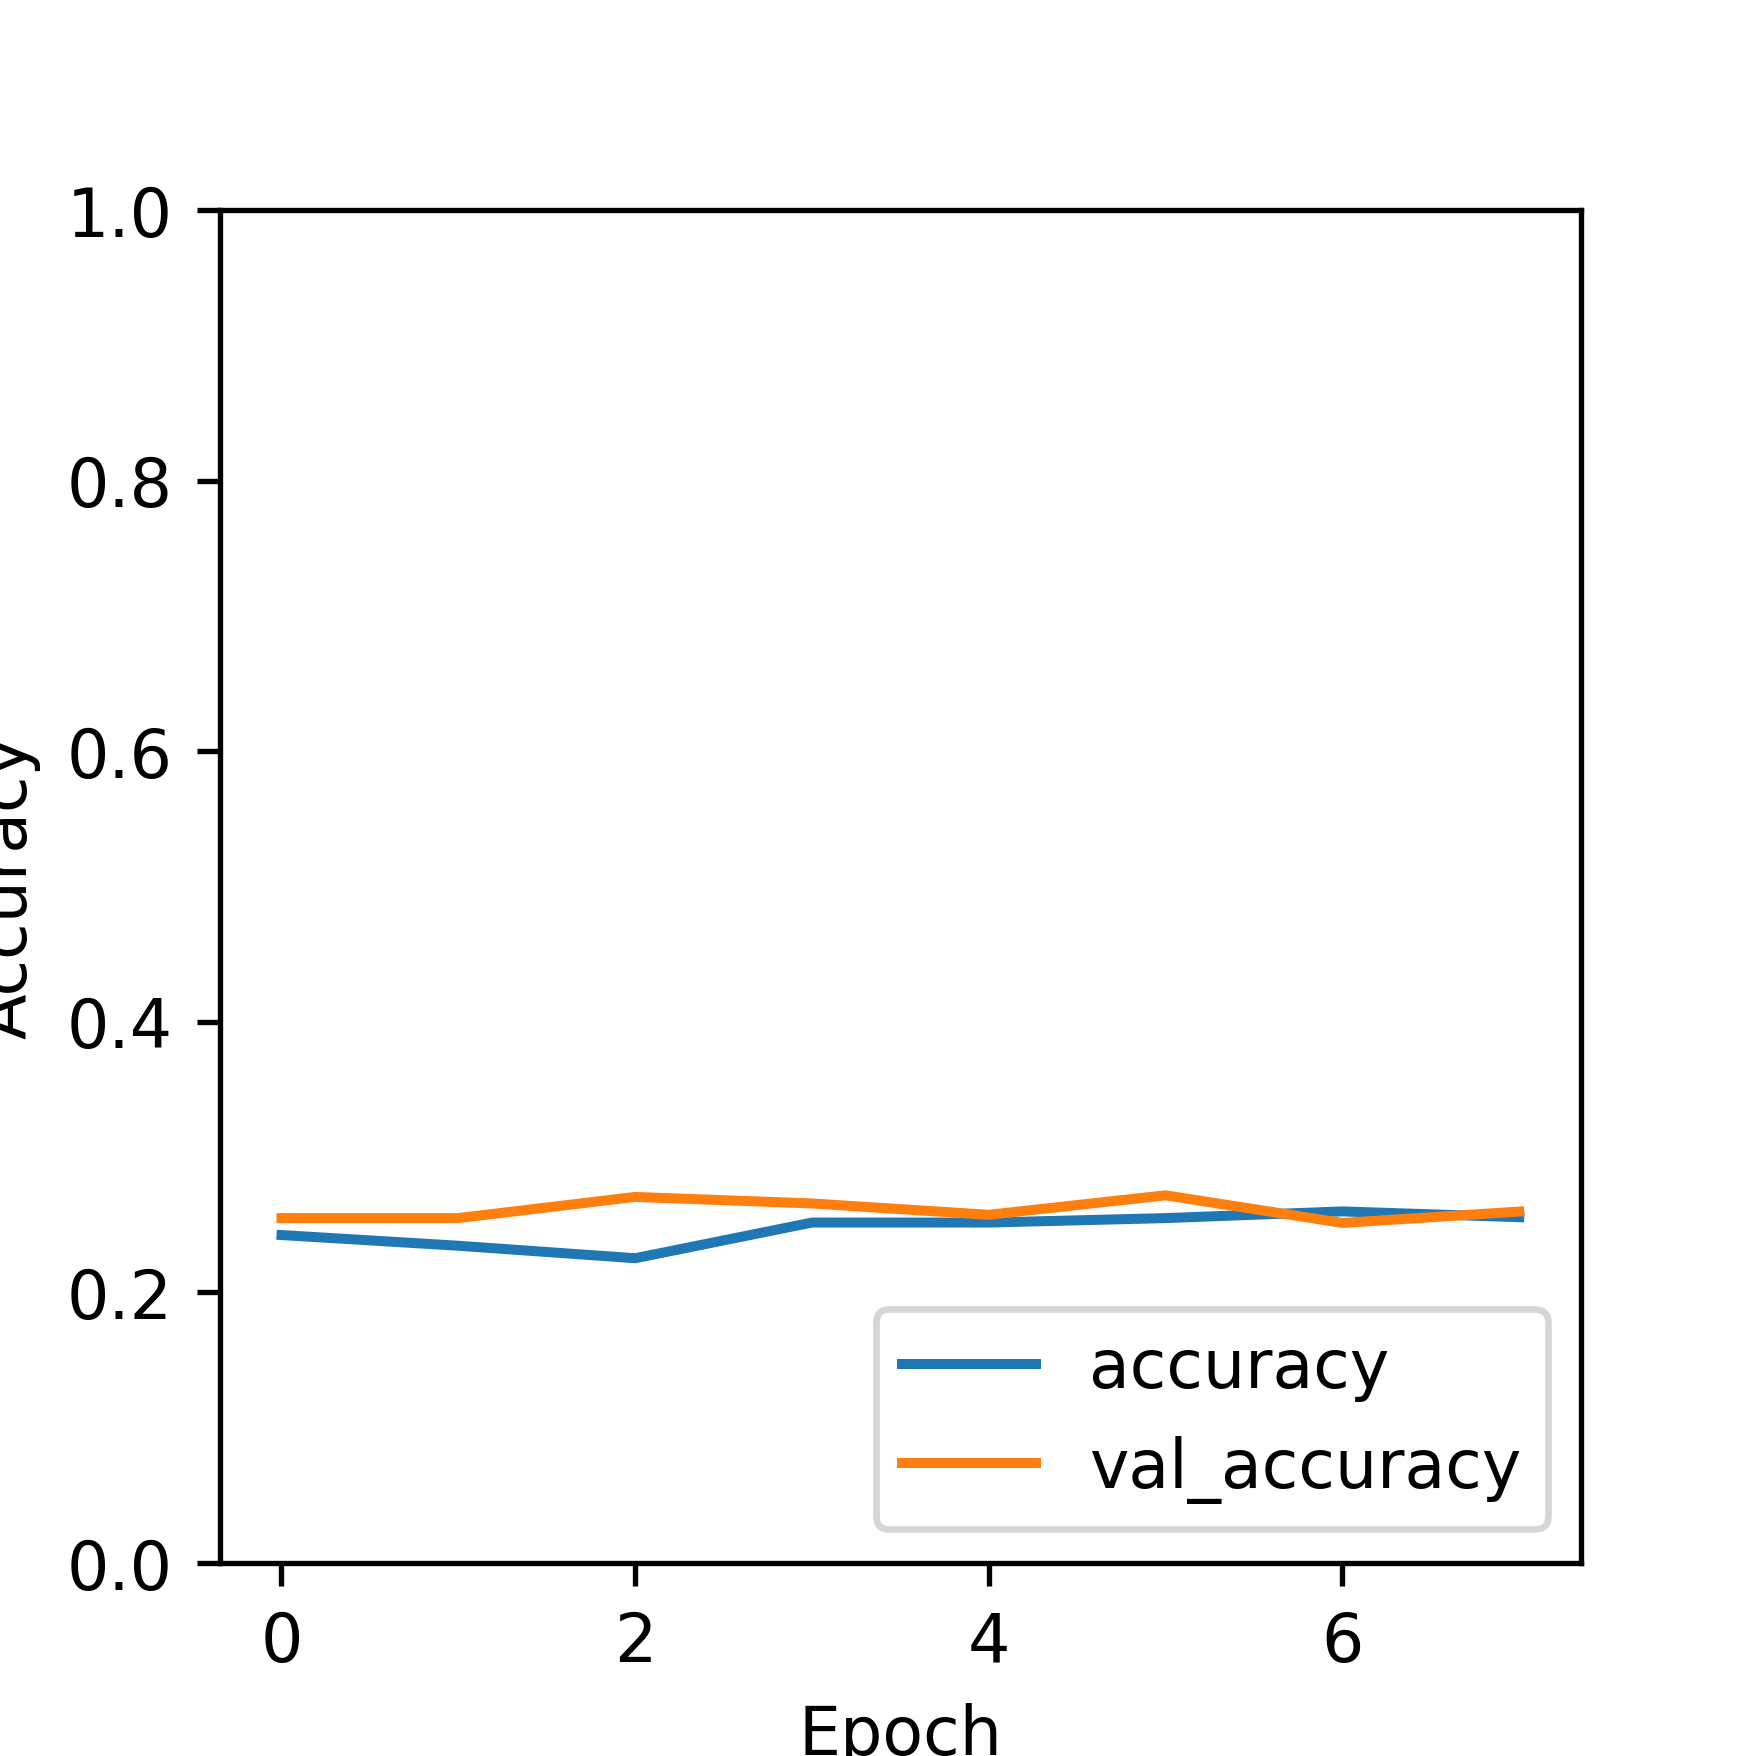
\includegraphics[width=.5\textwidth]{assets/results/preMELD.vgg/vgg16_finetune/learning_history-acc.png}\hfill
	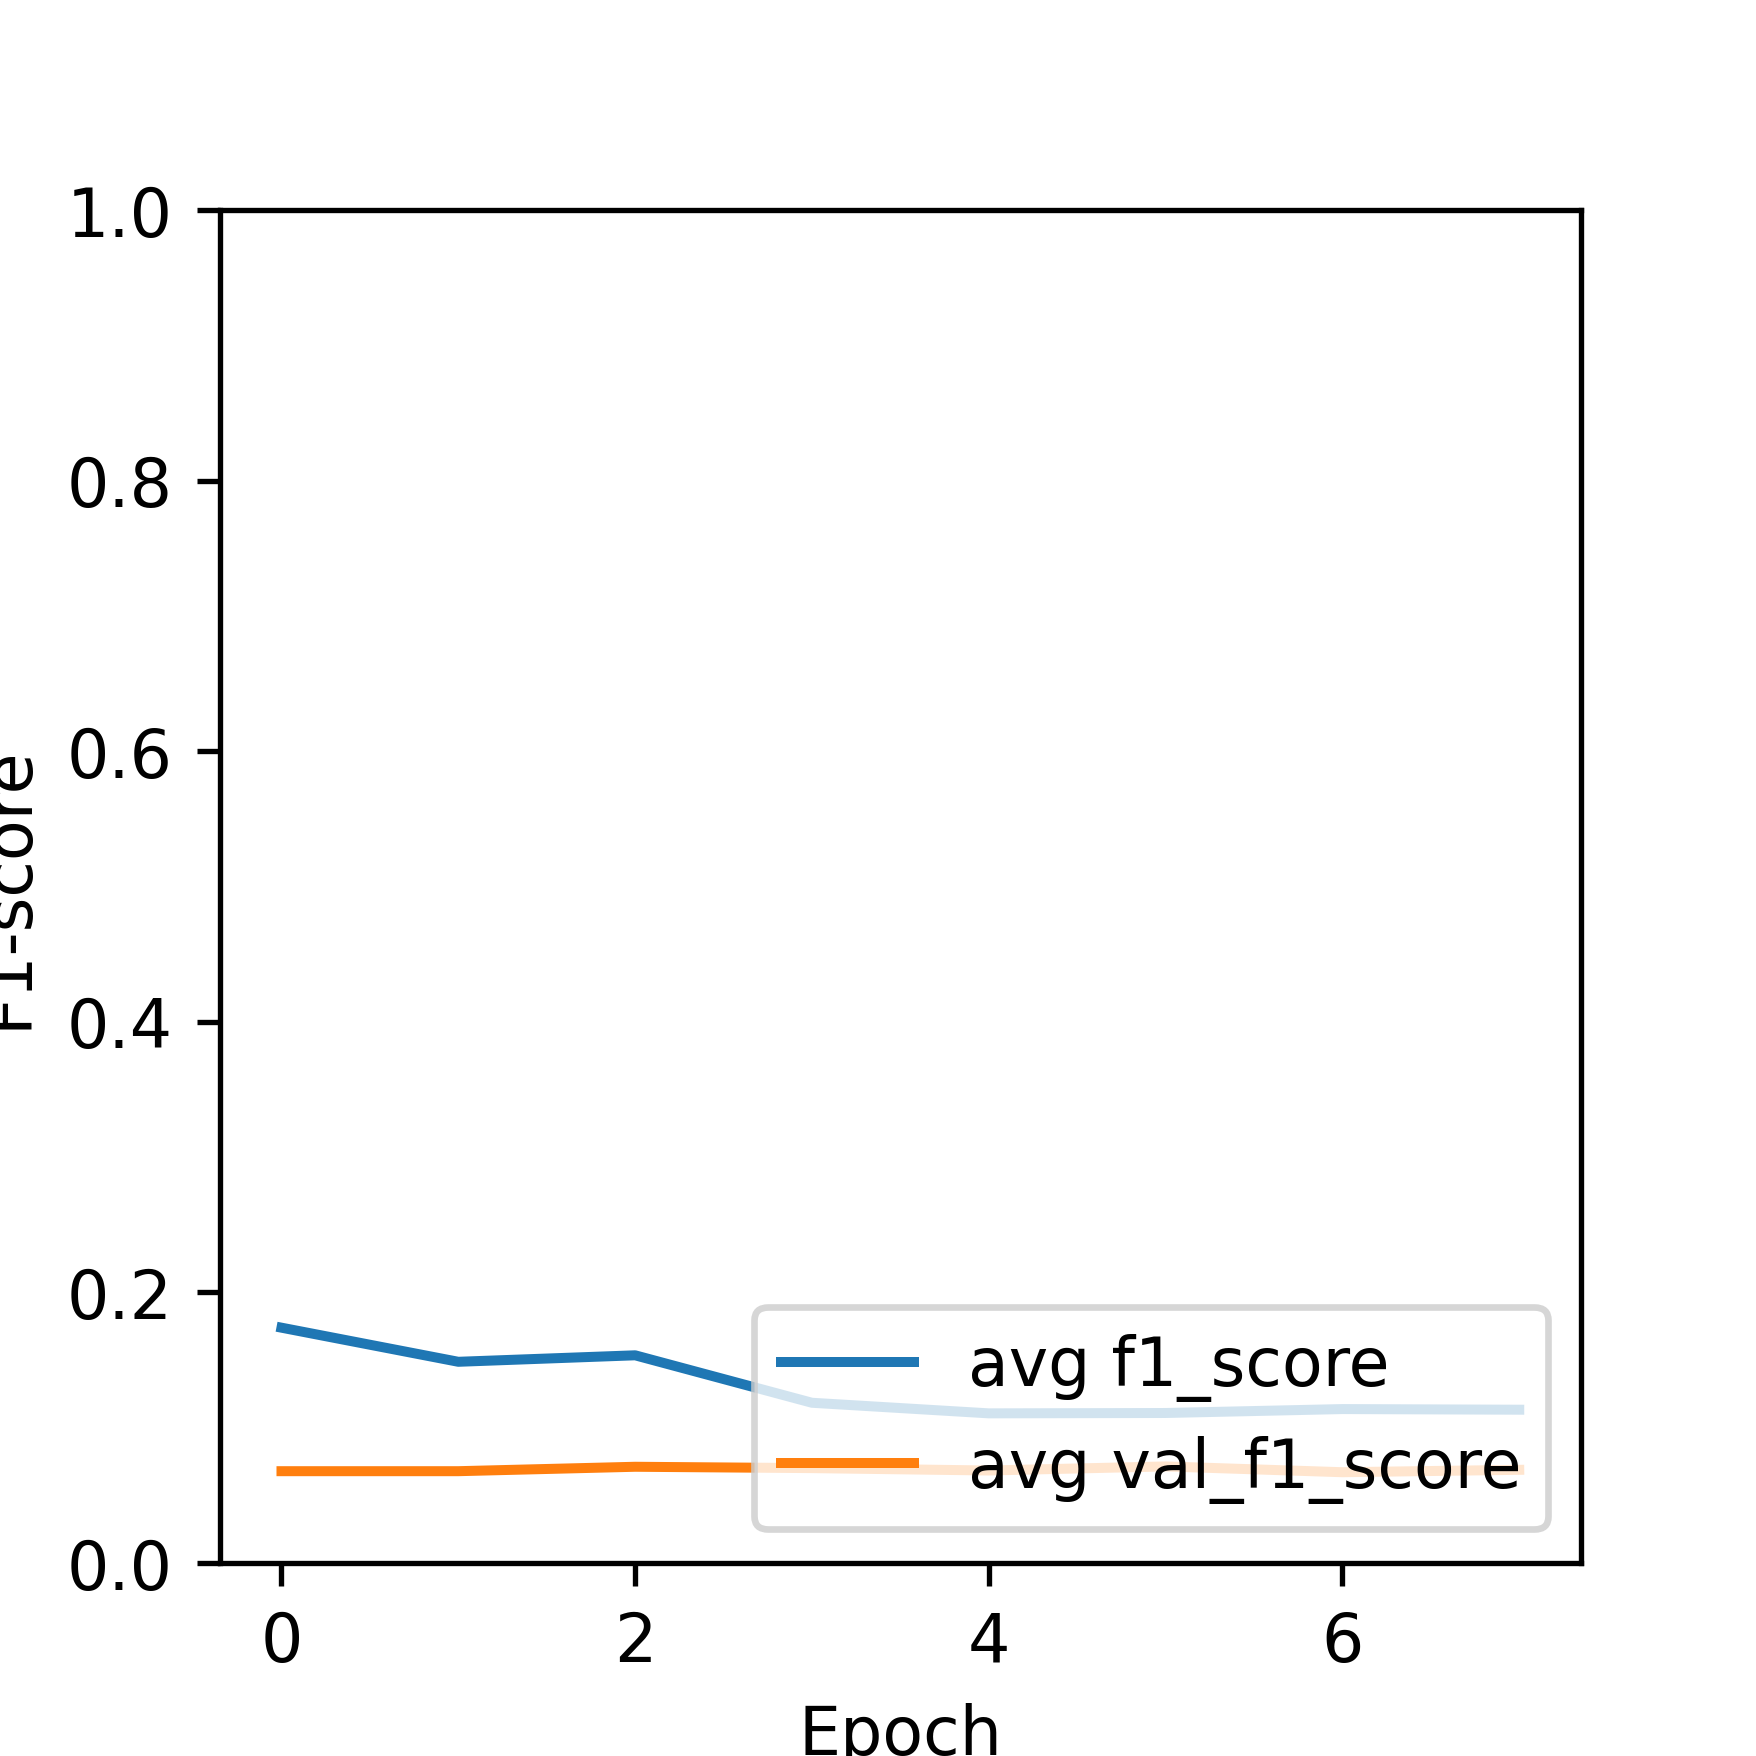
\includegraphics[width=.5\textwidth]{assets/results/preMELD.vgg/vgg16_finetune/learning_history-f1_score.png}\hfill
	\caption{$F_1$ figures are from average from all $F_1^c$}
	\label{fig:figure12}
\end{figure}

\begin{figure}[H]
	\centering
	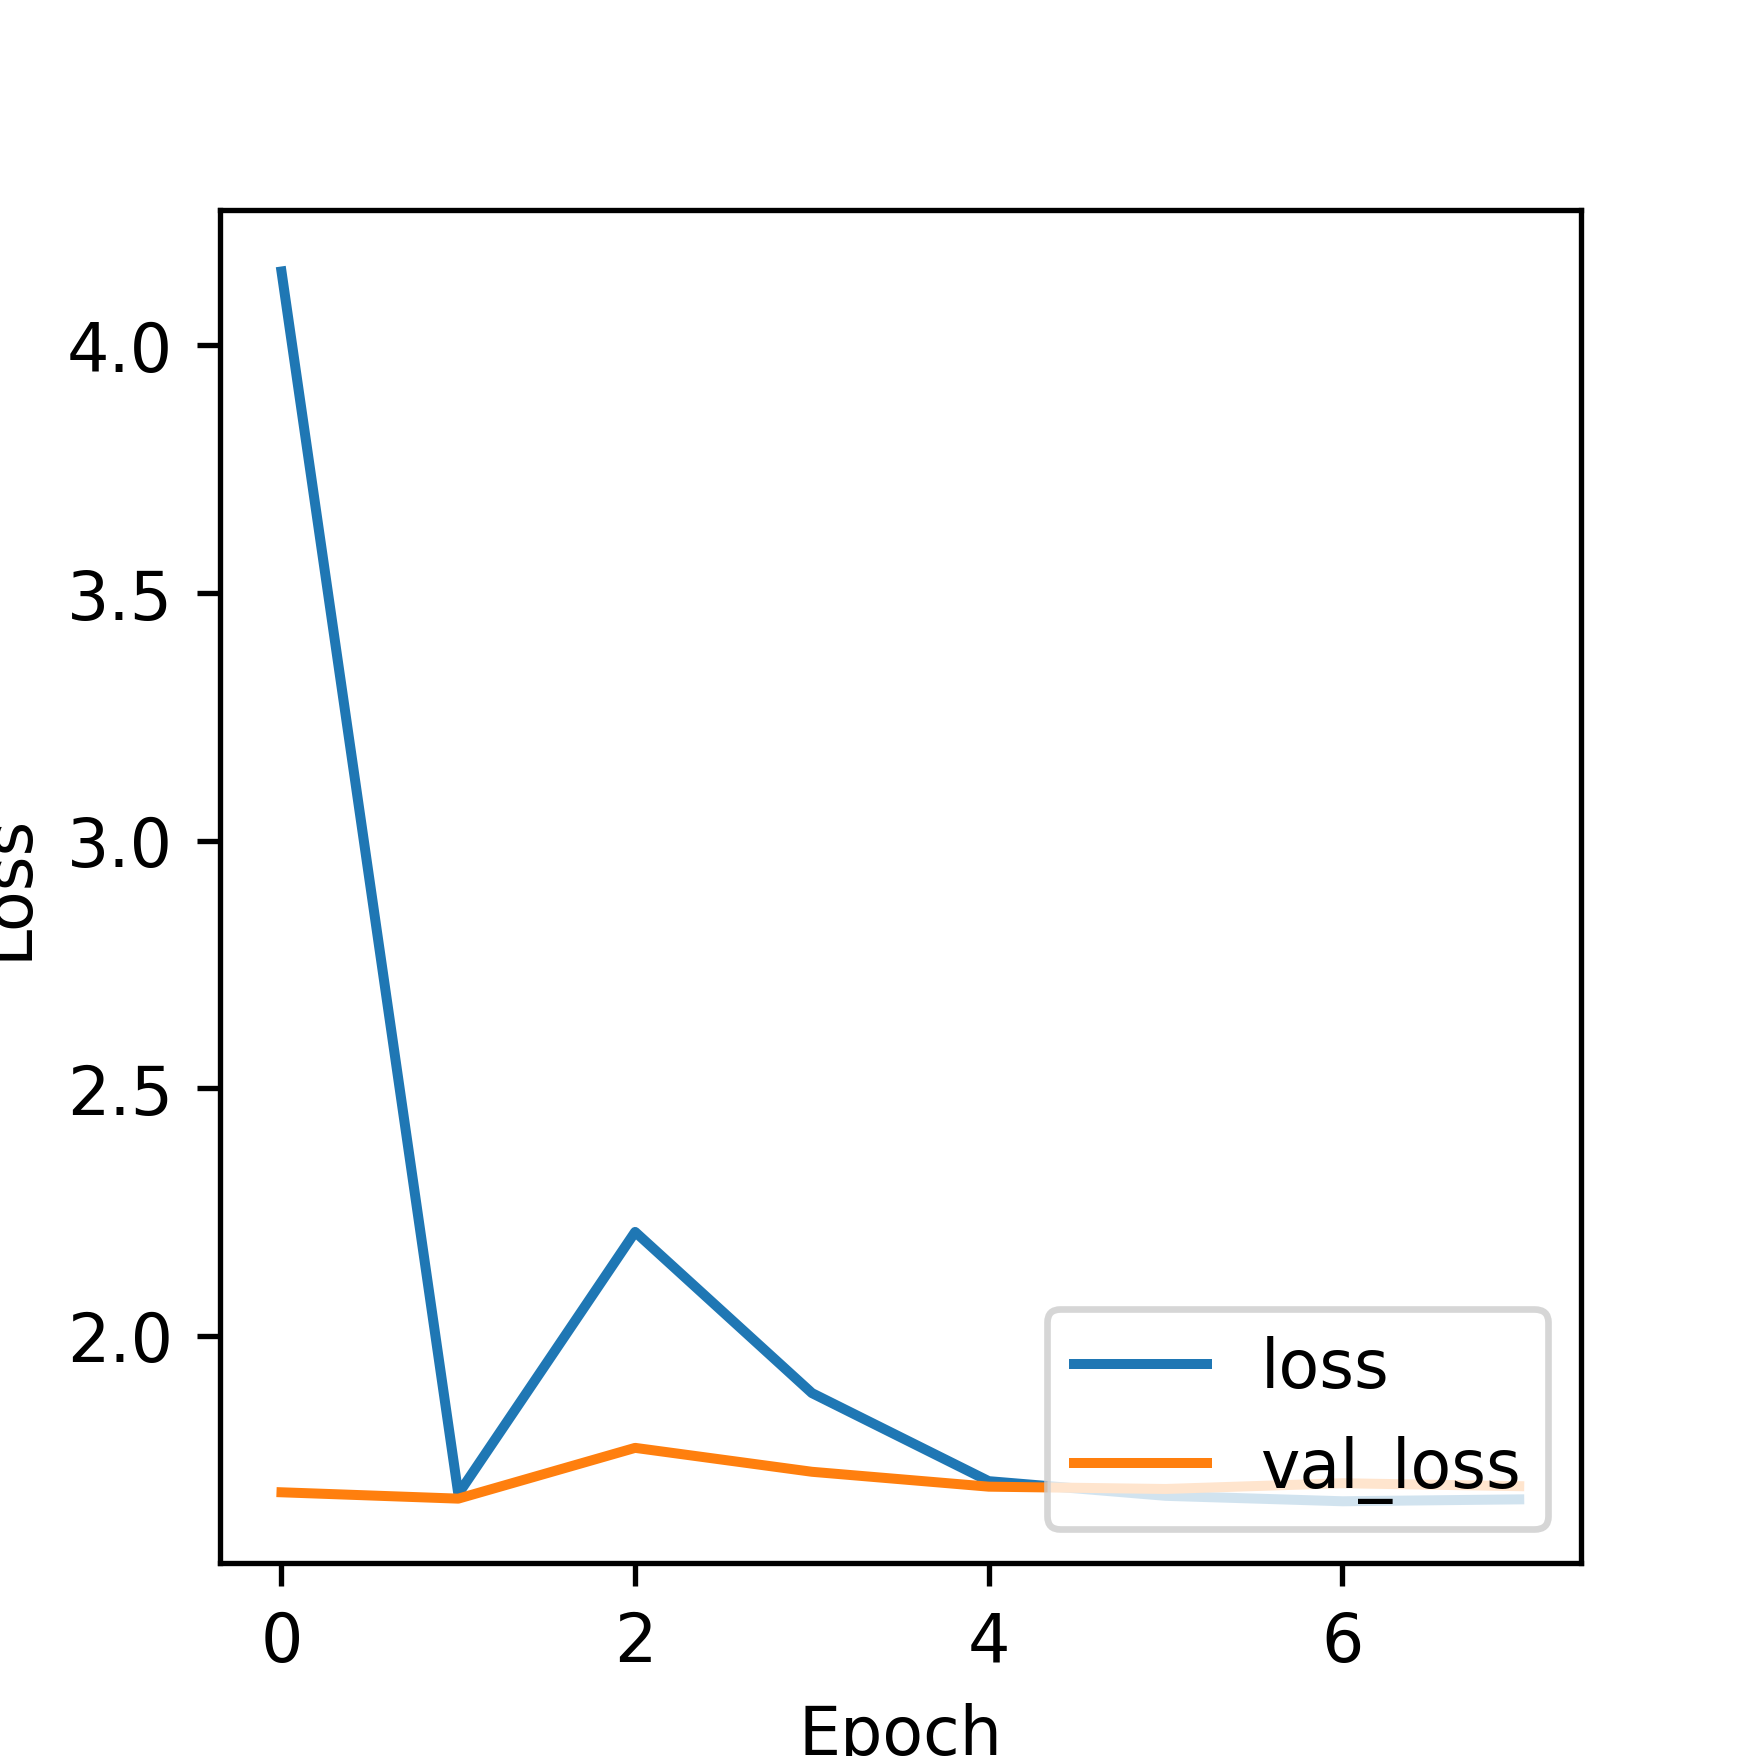
\includegraphics[width=.5\textwidth]{assets/results/preMELD.vgg/vgg16_finetune/learning_history-loss.png}
	
	\label{fig:figure11}
\end{figure}

\begin{figure}[H]
	\centering
	\includegraphics[width=.95\textwidth]{assets/results/preMELD.vgg/vgg16_finetune/confusion_matrix.png}
	
	\label{fig:cm5}
\end{figure}


